\documentclass[aspectratio=169,11pt]{beamer}

% =========================
% Theme
% =========================
\usetheme{Madrid}

% =========================
% Red Color Theme
% =========================
\definecolor{darkred}{RGB}{120,0,0}
\definecolor{lightred}{RGB}{180,30,30}
\definecolor{softred}{RGB}{245,235,235}

\setbeamercolor{title}{fg=white,bg=darkred}
\setbeamercolor{frametitle}{fg=white,bg=darkred}

\setbeamercolor{structure}{fg=darkred}

\setbeamercolor{section in toc}{fg=darkred}
\setbeamercolor{subsection in toc}{fg=lightred}

\setbeamercolor{block title}{bg=darkred,fg=white}
\setbeamercolor{block body}{bg=softred,fg=black}

\setbeamercolor{item}{fg=darkred}

\setbeamercolor{palette primary}{bg=darkred,fg=white}
\setbeamercolor{palette secondary}{bg=lightred,fg=white}
\setbeamercolor{palette tertiary}{bg=darkred,fg=white}
\setbeamercolor{palette quaternary}{bg=black,fg=white}

\setbeamercolor{footline}{bg=darkred,fg=white}

% =========================
% Remove navigation symbols
% =========================
\setbeamertemplate{navigation symbols}{}
\setbeamertemplate{caption}[numbered]

% =========================
% Packages
% =========================
\usepackage[T1]{fontenc}
\usepackage[utf8]{inputenc}
\usepackage{lmodern}
\usepackage{amsmath,amssymb,bm}
\usepackage{booktabs}
\usepackage{graphicx}
\usepackage{hyperref}
\usepackage{tikz}
\usetikzlibrary{positioning,arrows.meta}

\graphicspath{{assets/images/}{assets/logos/}}

% =========================
% Custom Commands
% =========================
% Command to add references/sources at the bottom of a slide without footnote markers
\newcommand{\source}[1]{\let\thefootnote\relax\footnotetext{\tiny \textcolor{gray}{Reference: #1}}}

% BibLaTeX Setup
\usepackage[backend=biber,style=authoryear,sorting=nyt,maxcitenames=2]{biblatex}
\addbibresource{bibliography/references.bib}

% Remove bibliography icon
\setbeamertemplate{bibliography item}{}

% =========================
% Custom Citation Command
% =========================
\usepackage[absolute,overlay]{textpos}
\DeclareCiteCommand{\myjournalortitle}
  {\usebibmacro{prenote}}
  {\iffieldundef{journaltitle}
     {\printfield{title}}
     {\printfield{journaltitle}}}
  {\multicitedelim}
  {\usebibmacro{postnote}}

\newcommand{\rightcite}[1]{%
  \begin{textblock*}{0.7\paperwidth}(0.29\paperwidth,0.92\paperheight)
  \raggedleft
  \tiny \textcolor{gray}{\citename{#1}{author}, \textit{\myjournalortitle{#1}} (\citeyear{#1})}
  \end{textblock*}%
}

% =========================
% Title Info
% =========================
\title[Active Droplet Dynamics]{Memory-Driven Dynamics of Self-Propelled Droplets}

\subtitle{
Experimental Analysis and PDE--SDE Modelling
}

\author{Pranav Deepak Shinde}

\institute{
Department of Physics\\
National Institute of Technology Karnataka, Surathkal
}

\date{JUNE 2026}

% =========================
% Footer
% =========================
\setbeamertemplate{footline}
{
    \leavevmode
    \hbox{
        \begin{beamercolorbox}[wd=.33\paperwidth,ht=2.5ex,dp=1ex,center]{author in head/foot}
            \insertshortauthor
        \end{beamercolorbox}

        \begin{beamercolorbox}[wd=.34\paperwidth,ht=2.5ex,dp=1ex,center]{title in head/foot}
            \insertshorttitle
        \end{beamercolorbox}

        \begin{beamercolorbox}[wd=.33\paperwidth,ht=2.5ex,dp=1ex,right]{date in head/foot}
            \insertframenumber{} / \inserttotalframenumber
            \hspace{2ex}
        \end{beamercolorbox}
    }
}

% =========================
% Begin Document
% =========================
\begin{document}

\input{sections/00-title}
\input{sections/01-outline}
\section{Introduction}
%================================================
\begin{frame}{Active Matter Systems}

	\begin{columns}[T]

		%-----------------------------------
		\column{0.38\textwidth}

		\begin{itemize}
			\item Active matter consists of entities that consume energy and convert it into motion.

			\item Active systems are found in both living and synthetic systems.

			\item These systems exhibit persistence, collective behaviour, and non-equilibrium transport.
		\end{itemize}

		\vspace{-0.2cm}

		\begin{alertblock}{Motivating Question}
			What mechanism allows active droplets to remember where they have been?
		\end{alertblock}

		%-----------------------------------
		\column{0.58\textwidth}

		\begin{block}{Examples of Active Matter}

			\centering

			\begin{tabular}{ccc}

				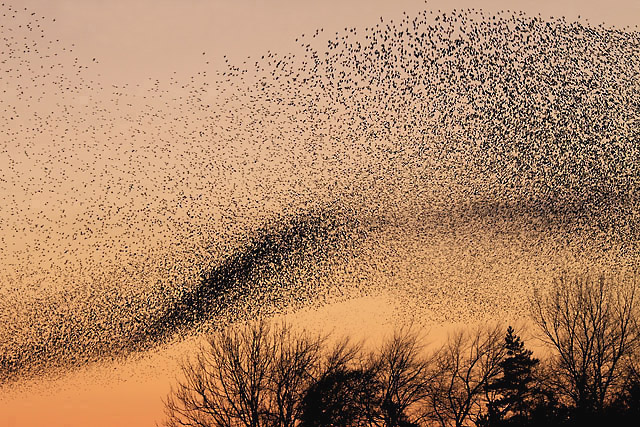
\includegraphics[height=1.9cm]{Starling_murmuration.jpg}
				 &
				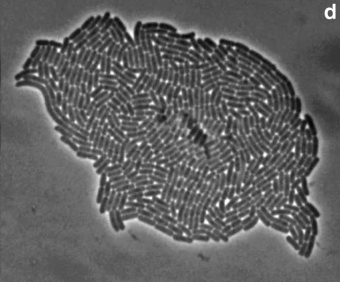
\includegraphics[height=1.9cm]{bacteria.png}
				 &
				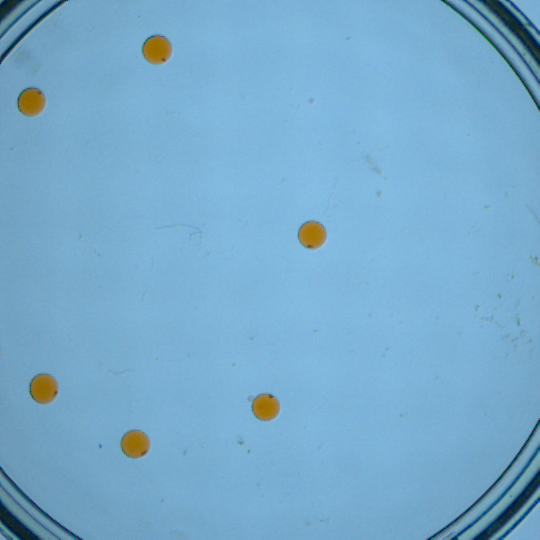
\includegraphics[height=1.9cm]{lab_droplet_image.png}

				\\[0.05cm]

				{\small Bird flock}
				 &
				{\small Bacteria}
				 &
				{\small Active droplet}
			\end{tabular}

		\end{block}
		\vspace{0.1cm}
		{\tiny
			\textbf{Image Sources}
			\begin{itemize}
				\item Bird flock: \emph{A murmuration of starlings at Gretna}, adapted from Walter Baxter (2011), Wikimedia Commons.

				\item Bacterial colony: Growing \textit{E. coli} microcolony exhibiting active-nematic ordering, adapted from Dell'Arciprete \textit{et al.}, \emph{Nature Communications} (2018).

				\item Active droplet: Self-propelled Belousov--Zhabotinsky (BZ) droplet driven by chemical oscillations and Marangoni flow, Nonlinear Dynamics Laboratory, NITK.
			\end{itemize}
		}
	\end{columns}


\end{frame}
%================================================

%================================================
\begin{frame}{Why Active Droplets?}

	\begin{columns}[T]

		%-----------------------------------
		\column{0.48\textwidth}

		\centering

		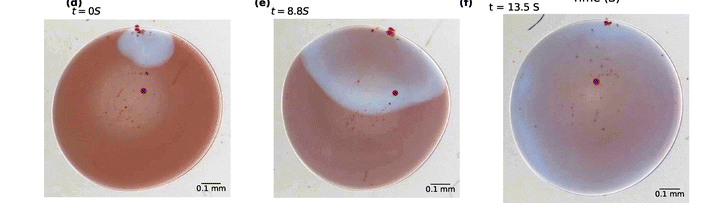
\includegraphics[width=\linewidth]{BZ_active_droplet.png}

		\vspace{0.15cm}

		{\scriptsize
			BZ active droplet exhibiting internal chemical-wave dynamics.
			Adapted from Meshram and Shajahan (2025).
		}

		%-----------------------------------
		\column{0.48\textwidth}

		\begin{block}{Key Features}

			\begin{itemize}

				\item Simple and controllable active matter system.

				\item Self-propelled through internally generated chemical activity.

				\item Continuously modifies its surrounding environment.

				\item Provides a natural platform for studying memory and feedback effects.

			\end{itemize}

		\end{block}

	\end{columns}

	\vspace{0.2cm}

	\begin{alertblock}{Hypothesis}
		The self-generated chemical field may retain information about previously visited locations and influence future motion.
	\end{alertblock}

\end{frame}
%================================================

%------------------------------------------------
\begin{frame}{Observation: Self-Avoiding Motion}

	\begin{columns}[T]

		\column{0.60\textwidth}

		\centering
		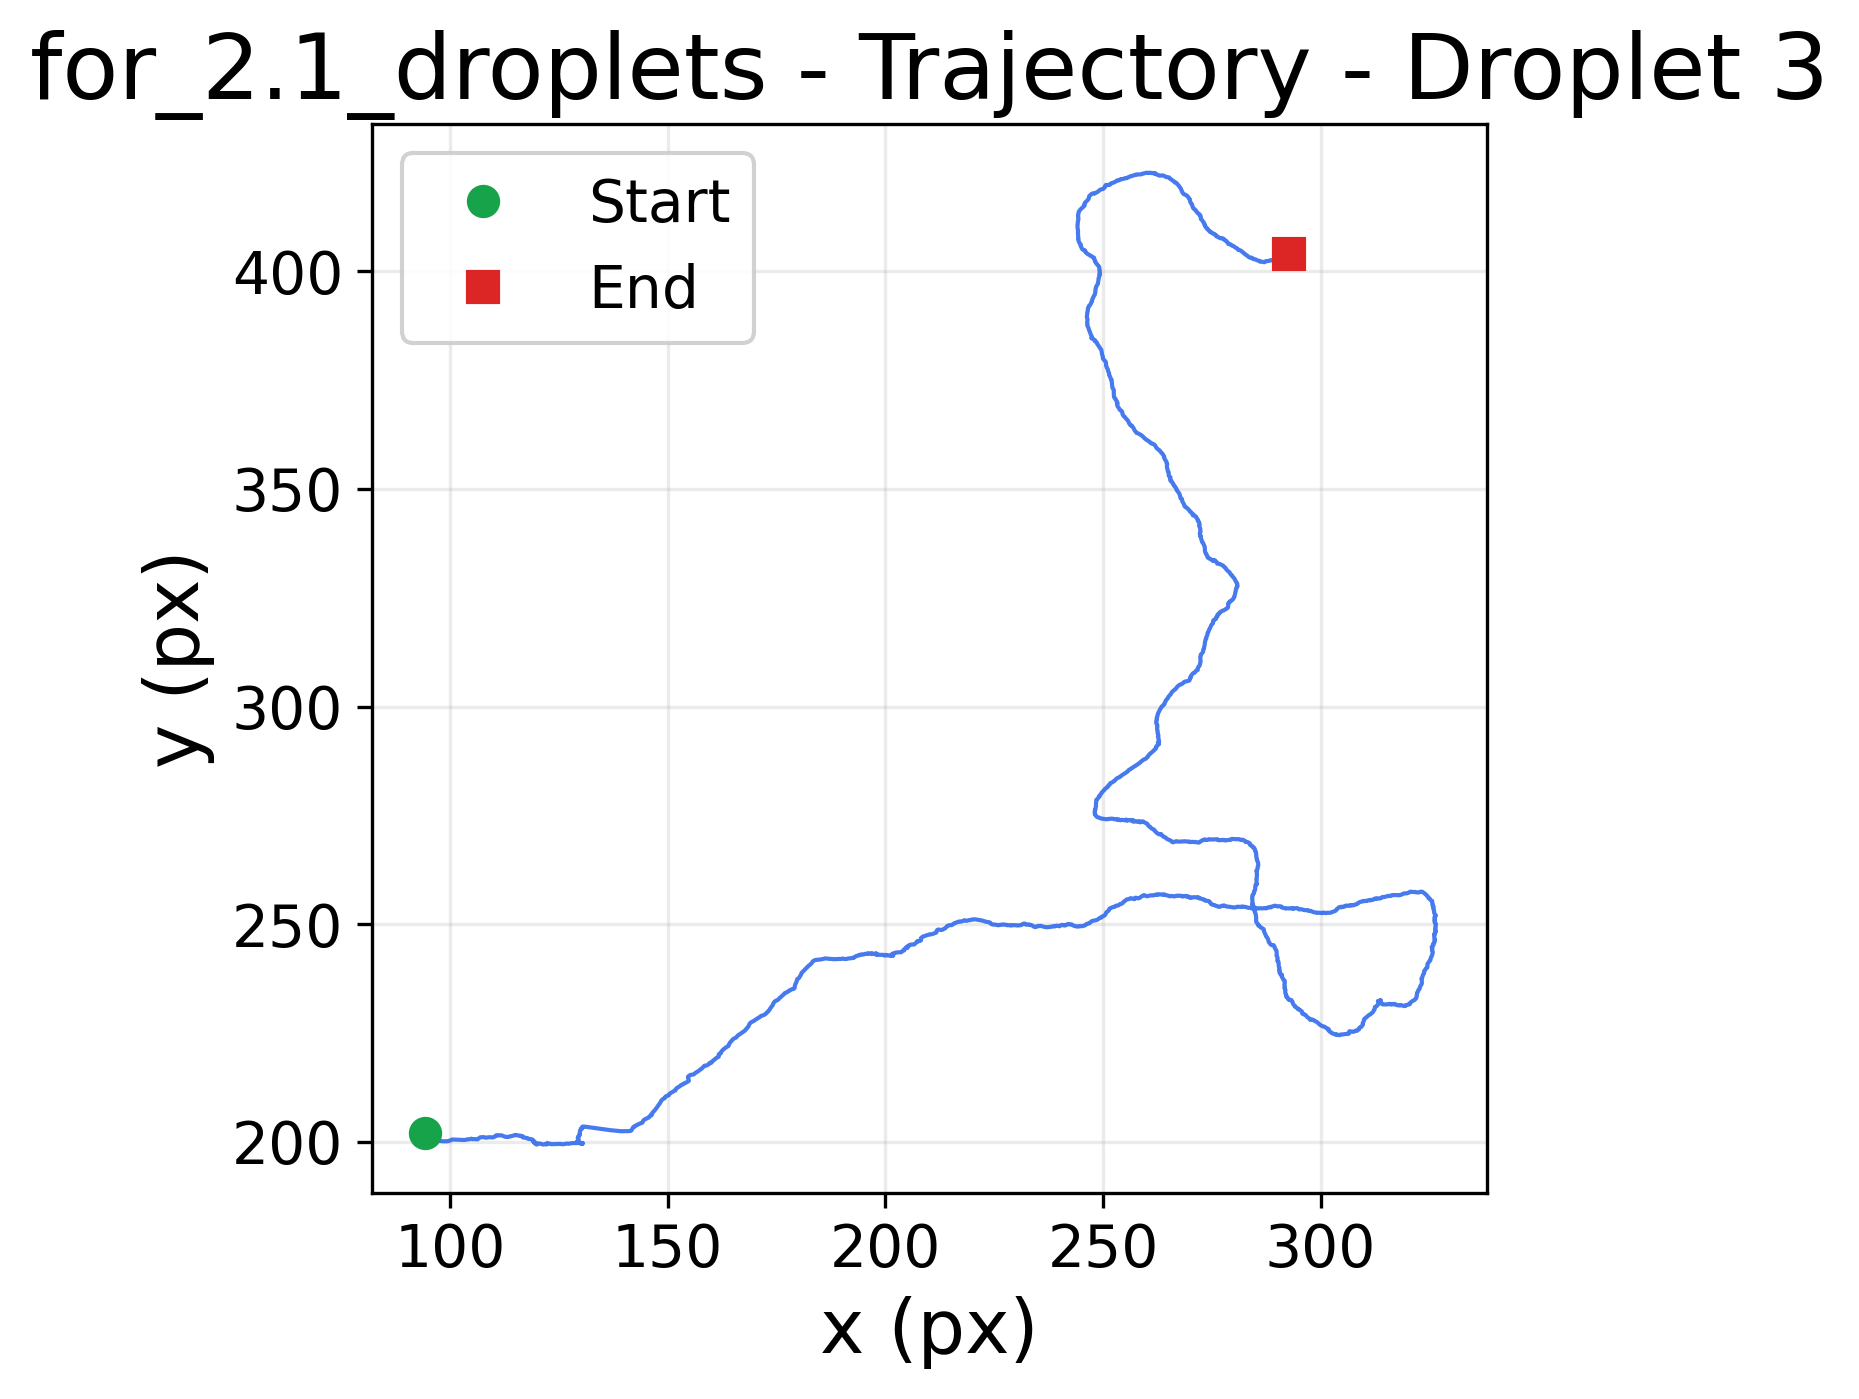
\includegraphics[height=0.62\textheight]{for_2.1_droplets_droplet_3_trajectory.png}

		\column{0.40\textwidth}

		\begin{block}{Observation}
			The droplet tends to avoid regions it has previously visited.
		\end{block}

		\vspace{0.2cm}

		\begin{itemize}
			\item Motion is not purely random.
			\item Trajectories exhibit self-avoidance.
			\item Past motion appears to influence future motion.
		\end{itemize}

	\end{columns}

	\vspace{0.15cm}

	\begin{alertblock}{Research Question}
		What mechanism allows the droplet to remember where it has been?
	\end{alertblock}

\end{frame}
%------------------------------------------------
\begin{frame}{A Possible Explanation: Memory}

	\centering

	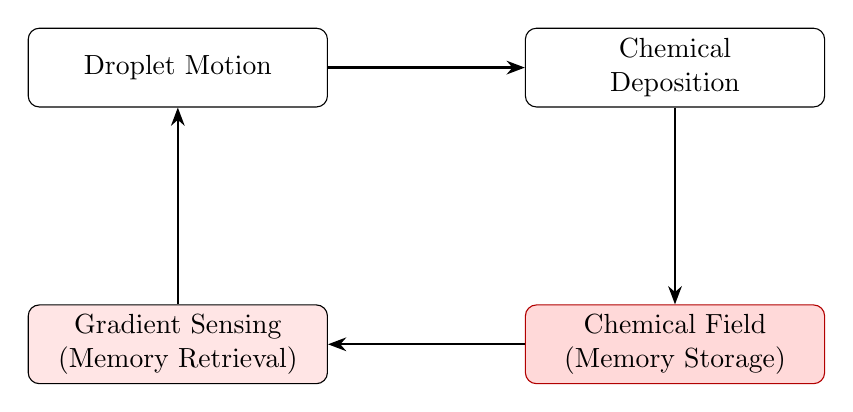
\begin{tikzpicture}[
			node distance=2.5cm,
			every node/.style={
					draw,
					rounded corners,
					align=center,
					minimum width=3.8cm,
					minimum height=1cm
				},
			>=Stealth
		]

		\node (motion) {Droplet Motion};

		\node (deposit) [right=of motion]
		{Chemical\\Deposition};

		\node (memory) [below=of deposit,
			fill=red!15,
			draw=red!70!black]
		{Chemical Field\\(Memory Storage)};

		\node (retrieve) [left=of memory,
			fill=red!10]
		{Gradient Sensing\\(Memory Retrieval)};

		\draw[->,thick] (motion) -- (deposit);
		\draw[->,thick] (deposit) -- (memory);
		\draw[->,thick] (memory) -- (retrieve);
		\draw[->,thick] (retrieve) -- (motion);

	\end{tikzpicture}

	\vspace{0.5cm}

	\begin{alertblock}{Hypothesis}
		The droplet deposits a chemical trail that stores information about previously visited locations. By sensing gradients in this field, the droplet's future motion becomes influenced by its past motion.
	\end{alertblock}

\end{frame}

%------------------------------------------------
\begin{frame}{Research Question}

	\begin{center}

		\Large
		Does the observed self-avoidance indicate memory-driven dynamics?

	\end{center}

	\vspace{0.5cm}

	\begin{block}{Questions}
		\begin{enumerate}
			\item Does the droplet retain information about its past motion?
			\item Can this memory be quantified from trajectory data?
			\item Can a memory-driven model reproduce the observed behaviour?
		\end{enumerate}
	\end{block}

\end{frame}

%------------------------------------------------
\begin{frame}{How Do We Quantify Memory?}

	\centering

	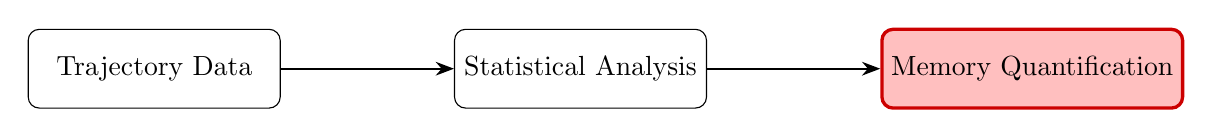
\begin{tikzpicture}[
			node distance=2.2cm,
			every node/.style={
					draw,
					rounded corners,
					align=center,
					minimum width=3.2cm,
					minimum height=1cm
				},
			>=Stealth
		]

		\node (traj) {Trajectory Data};

		\node (stats) [right=of traj]
		{Statistical Analysis};

		\node (memory) [right=of stats,
			fill=red!25,
			draw=red!80!black,
			very thick]
		{Memory Quantification};

		% \node (memory) [right=of stats,
		% fill=red!15]
		% {Memory Quantification};

		\draw[->,thick] (traj) -- (stats);
		\draw[->,thick] (stats) -- (memory);

	\end{tikzpicture}

	\vspace{0.9cm}

	\begin{center}
		\large
		From observed trajectories, we extract statistical signatures of memory.
	\end{center}
	\begin{columns}
		\column{0.4\textwidth}

		\begin{block}{Transport Characterization}
			\begin{itemize}
				\item MSD
				      {\small \\How far does the droplet travel?}
				      % \item MSD \\- How far does the droplet travel?
				\item Local MSD Exponent
					      {\small \\Does transport change with time?}
			\end{itemize}
		\end{block}

		\column{0.4\textwidth}

		\begin{alertblock}{Memory Characterization}
			% \begin{block}{Memory Characterization}
			\begin{itemize}
				\item Velocity Autocorrelation
					      {\small \\How long is velocity remembered?}

				\item Orientation Correlation
					      {\small \\How long is direction remembered?}

			\end{itemize}
		\end{alertblock}

	\end{columns}


\end{frame}

\begin{frame}{Research Strategy and Methodology}

	\centering

	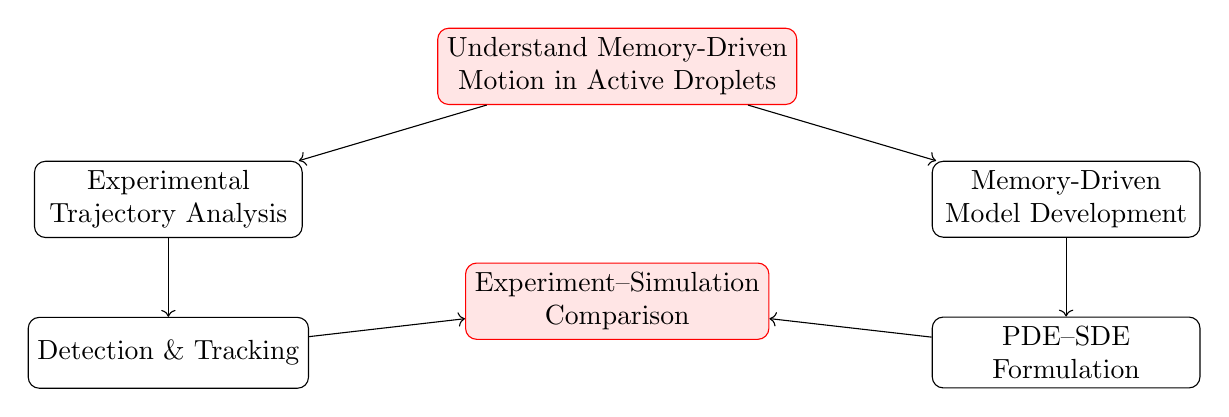
\begin{tikzpicture}[
			node distance=1.cm,
			every node/.style={
					draw,
					rounded corners,
					align=center,
					minimum width=3.4cm,
					minimum height=0.9cm
				}
		]

		\node[fill=red!10,draw=red] (goal)
		{Understand Memory-Driven\\Motion in Active Droplets};

		\node[below left=of goal,xshift=-1cm] (exp)
		{Experimental\\Trajectory Analysis};

		\node[below right=of goal,xshift=1cm] (model)
		{Memory-Driven\\Model Development};

		\node[below=of exp] (track)
		{Detection \& Tracking};

		\node[below=of model] (pde)
		{PDE--SDE\\Formulation};

		\node[below=2.0cm of goal,fill=red!10,draw=red] (compare)
		{Experiment--Simulation\\Comparison};

		\draw[->] (goal)--(exp);
		\draw[->] (goal)--(model);

		\draw[->] (exp)--(track);
		\draw[->] (model)--(pde);

		\draw[->] (track)--(compare);
		\draw[->] (pde)--(compare);

	\end{tikzpicture}

	\vspace{0.3cm}

	\begin{alertblock}{Objective}
		Combine experimental trajectory analysis with a memory-driven
		PDE--SDE model to identify and reproduce memory signatures
		in active droplet motion.
	\end{alertblock}

\end{frame}

\section{Methodology}


%================================================
% \begin{frame}{Methodology Overview}

% 	\centering

% 	\begin{tikzpicture}[
% 			node distance=0.4cm,
% 			every node/.style={
% 					draw,
% 					rounded corners,
% 					align=center,
% 					minimum width=3.8cm,
% 					minimum height=0.8cm
% 				},
% 			>=Stealth
% 		]

% 		%-----------------------------------
% 		% Experimental branch

% 		\node (video)
% 		at (-4,0)
% 		{Experimental Videos};

% 		\node (track)
% 		at (-4,-1.5)
% 		{Detection \& Tracking};

% 		\node (traj)
% 		at (-4,-3)
% 		{Droplet Trajectories};

% 		%-----------------------------------
% 		% Model branch

% 		\node (model)
% 		at (4,0)
% 		[fill=red!10,draw=red!70!black]
% 		{Memory-Driven Model};

% 		\node (pde)
% 		at (4,-1.5)
% 		{PDE--SDE Formulation};

% 		\node (sim)
% 		at (4,-3)
% 		{Numerical Simulation};

% 		%-----------------------------------
% 		% Comparison

% 		\node (compare)
% 		at (0,-4.8)
% 		[fill=red!15,draw=red!70!black]
% 		{Experiment--Simulation Comparison};

% 		%-----------------------------------
% 		% Arrows

% 		\draw[->,thick] (video) -- (track);
% 		\draw[->,thick] (track) -- (traj);

% 		\draw[->,thick] (model) -- (pde);
% 		\draw[->,thick] (pde) -- (sim);

% 		\draw[->,thick] (traj) -- (compare);
% 		\draw[->,thick] (sim) -- (compare);

% 	\end{tikzpicture}
% \end{frame}
%================================================
\begin{frame}{Experimental System}

	\begin{columns}

		\column{0.55\textwidth}

		\begin{itemize}
			\item Self-propelled Belousov--Zhabotinsky (BZ) droplets in a monoolein--squalane oil medium.
			\item Droplet diameter: $\approx 1.75\,\mathrm{mm}$.
			\item Videos recorded using a CMOS camera at 5 fps.
			\item Spatial resolution: $0.06\,\mathrm{mm}$ per pixel.

		\end{itemize}

		\column{0.45\textwidth}

		\centering

		% Replace with experimental setup image
		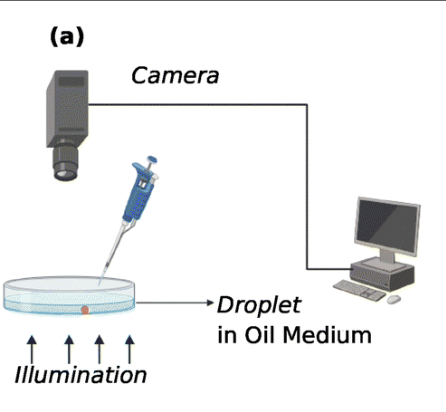
\includegraphics[height=0.58\textheight]{camera_setup_image.png}

		\vspace{0.2cm}
		{\scriptsize Experimental setup for recording active droplet trajectories. Adapted from Meshram and Shajahan (2026).\par}
	\end{columns}
	\rightcite{D5SM01187F}

\end{frame}

%================================================
%================================================
\begin{frame}{Trajectory Extraction}

	\vspace{-0.2cm}

	\begin{columns}[T]

		%=========================================
		\column{0.48\textwidth}

		\begin{block}{YOLOv8 Detection and Tracking}

			\small

			\begin{itemize}
				\item Detect droplets in each frame.
				\item Assign persistent tracking IDs.
				\item Link detections across frames.
				\item Extract centroid coordinates.
				\item Reconstruct droplet trajectories.
			\end{itemize}

			\vspace{0.15cm}

			{\footnotesize
				Transfer learning using YOLOv8
				(369 training images, 96 validation images,
				50 epochs, resolution $640\times640$).
			}

		\end{block}

		\vspace{0.15cm}

		%=========================================
		\column{0.52\textwidth}

		\centering

		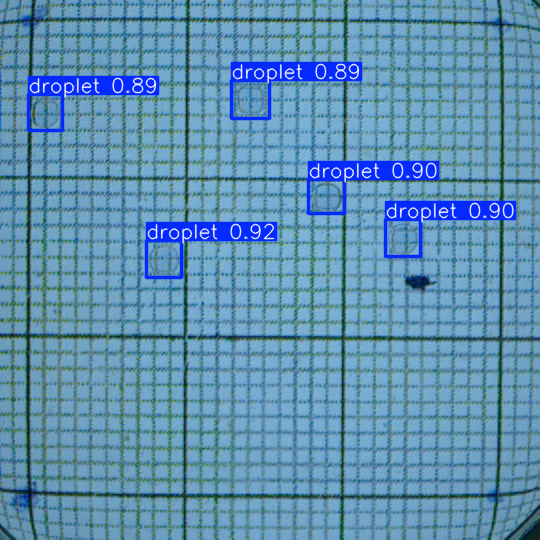
\includegraphics[height=0.55\textheight]{yolo_tracking_example.png}

		\vspace{0.1cm}

		{\tiny
			\begin{minipage}{0.9\linewidth}
				\centering
				YOLOv8 detection and tracking output.\\
				Bounding boxes and persistent tracking IDs\\
				enable trajectory reconstruction across video frames.
			\end{minipage}
		}
	\end{columns}

	\begin{alertblock}{Output}

		Tracked droplet trajectories used for
		transport and memory analysis.

	\end{alertblock}
\end{frame}
%================================================
\begin{frame}{From Trajectories to Memory Measures}

	\centering

	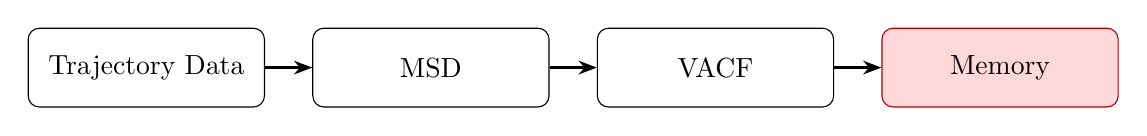
\begin{tikzpicture}[
			node distance=0.6cm,
			every node/.style={
					draw,
					rounded corners,
					align=center,
					minimum width=3cm,
					minimum height=1cm
				},
			> =Stealth
		]

		\node (traj) {Trajectory Data};

		\node (msd) [right=of traj]
		{MSD};

		\node (vacf) [right=of msd]
		{VACF};

		\node (memory) [right=of vacf,
			fill=red!15,
			draw=red!70!black]
		{Memory};

		\draw[->,thick] (traj) -- (msd);
		\draw[->,thick] (msd) -- (vacf);
		\draw[->,thick] (vacf) -- (memory);

	\end{tikzpicture}

	\vspace{0.6cm}

	\begin{columns}

		\column{0.4\textwidth}

		\begin{block}{Transport Measures}
			\begin{itemize}
				\item Mean Squared Displacement (MSD)
				\item Local MSD Exponent
			\end{itemize}
		\end{block}

		\column{0.4\textwidth}

		\begin{alertblock}{Memory Measures}
			\begin{itemize}
				\item Velocity Autocorrelation Function (VACF)
				\item Orientation Correlation Function (OCF)
			\end{itemize}
		\end{alertblock}

	\end{columns}

\end{frame}
\begin{frame}{Transport Characterization}

	\begin{columns}[T]

		%----------------------------------
		\column{0.48\textwidth}

		\begin{block}{Mean Squared Displacement (MSD)}

			\vspace{-0.05cm}

			\[
				\mathrm{MSD}(\tau)
				=
				\left\langle
				\|\mathbf{X}(t+\tau)-\mathbf{X}(t)\|^2
				\right\rangle
			\]

		\end{block}

		\begin{itemize}
			\item Measures spatial exploration.
			\item Identifies ballistic, diffusive, and anomalous transport.
			\item Used to estimate transport behavior.
		\end{itemize}

		%----------------------------------
		\column{0.48\textwidth}

		\begin{block}{Local MSD Exponent}

			\vspace{-0.05cm}

			\[
				\alpha(\tau)
				=
				\frac{d\log[\mathrm{MSD}(\tau)]}
				{d\log(\tau)}
			\]

		\end{block}

		\begin{itemize}
			\item Characterizes lag-dependent transport.
			\item $\alpha \approx 2$ : Ballistic motion
			\item $\alpha \approx 1$ : Normal diffusion
			\item $1<\alpha<2$ : Superdiffusion
		\end{itemize}

	\end{columns}

	\vspace{0.2cm}

	\begin{alertblock}{Physical Interpretation}
		MSD quantifies how far droplets travel, while the local exponent reveals how the transport regime evolves across timescales.
	\end{alertblock}

\end{frame}
\begin{frame}{Memory Characterization}

	\begin{columns}[T]

		%----------------------------------
		\column{0.4\textwidth}
		\vspace{-0.2cm}

		\begin{alertblock}{Velocity Autocorrelation Function (VACF)}

			\[
				C_v(\tau)
				=
				\frac{
					\left\langle
					\mathbf{v}(t)\cdot\mathbf{v}(t+\tau)
					\right\rangle}
				{
					\left\langle
					|\mathbf{v}(t)|^2
					\right\rangle}
			\]
		\end{alertblock}

		\vspace{0.05cm}

		\[
			C_v(\tau)\sim e^{-\tau/\tau_p}
		\]

		\begin{itemize}
			\item Measures velocity memory.
			\item Provides persistence time $\tau_p$.
		\end{itemize}

		%----------------------------------
		\column{0.4\textwidth}
		\vspace{-0.2cm}

		\begin{alertblock}{Orientation Correlation Function (OCF)}
			\vspace{-0.2cm}

			\[
				C_\theta(\tau)
				=
				\left\langle
				\cos[\theta(t+\tau)-\theta(t)]
				\right\rangle
			\]
			% \vspace{0.00005cm}
			% \vspace{-0.1cm}

		\end{alertblock}

		\vspace{0.05cm}

		\[
			C_\theta(\tau)\sim e^{-\tau/\tau_r}
		\]

		\begin{itemize}
			\item Measures directional memory.
			\item Provides rotational persistence time $\tau_r$.
		\end{itemize}

	\end{columns}

	\vspace{0.3cm}

	\begin{alertblock}{Physical Meaning}
		These observables quantify how long information about past velocity and direction persists.
	\end{alertblock}

\end{frame}

%================================================
\section{Memory-Driven Model}
\begin{frame}{Memory and Non-Markovian Dynamics}
	\vspace{-0.4cm}

	\begin{columns}[T]

		\column{0.48\textwidth}

		\begin{block}{Markovian Dynamics}
			\[
				P(X_{t+\Delta t}\mid X_t)
			\]

			\begin{itemize}
				\item Future depends only on the current state.
				\item No memory.
				\item Instantaneous response.
			\end{itemize}
			\vspace{-0.6cm}

			\[
				m\dot v(t)=-\gamma v(t)+\eta(t)
			\]
			\vspace{-0.8cm}

			\[
				K(t)=\gamma\delta(t)
			\]

		\end{block}

		\column{0.48\textwidth}

		\begin{block}{Non-Markovian Dynamics}
			\[
				P(X_{t+\Delta t}\mid X_t,X_{t-\tau},\ldots)
			\]

			\begin{itemize}
				\item Future depends on past history.
				\item Memory effects.
				\item Persistent correlations.
			\end{itemize}
			\vspace{-0.8cm}

			\[
				m\dot v(t)
				=
				-\int_0^t K(t-s)v(s)\,ds
				+\eta(t)
			\]
			\vspace{-0.8cm}

			\[
				K(t)=K_0e^{-t/\tau_m}
			\]

		\end{block}

	\end{columns}

	\vspace{0.3cm}

	\begin{alertblock}{Motivation}
		Finite VACF and OCF decay indicate that information about past
		velocity and orientation persists for a finite time, motivating
		a non-Markovian description with memory kernels.
	\end{alertblock}

\end{frame}
% % %================================================
% % \begin{frame}{From Markovian to Non-Markovian Dynamics}
% % 	\vspace{-0.4cm}

% % 	\begin{columns}[T]

% % 		%---------------------------------------
% % 		\column{0.48\textwidth}

% % 		\begin{block}{Markovian Dynamics}

% % 			Future motion depends only on the current state.
% % 			% \vspace{-0.2cm}
% % 			\vspace{-0.2cm}

% % 			\[
% % 				P(X_{t+\Delta t}|X_t)
% % 			\]

% % 			% \vspace{-0.5cm}
% % 			% \[
% % 			% 	m\dot v(t)
% % 			% 	=
% % 			% 	-\gamma v(t)+\eta(t)
% % 			% \]

% % 			\begin{itemize}
% % 				\item No memory.
% % 				\item Instantaneous response.
% % 				\item Brownian diffusion.
% % 			\end{itemize}

% % 		\end{block}

% % 		%---------------------------------------
% % 		\column{0.48\textwidth}

% % 		\begin{alertblock}{Non-Markovian Dynamics}

% % 			Future motion depends on past history.
% % 			% \vspace{-0.2cm}
% % 			\vspace{0.2cm}

% % 			\[
% % 				P(X_{t+\Delta t}|X_t,X_{t-\tau},\ldots)
% % 			\]

% % 			% \vspace{-0.7cm}

% % 			% \[
% % 			% 	m\dot v(t)
% % 			% 	=
% % 			% 	-\int_0^t K(t-s)v(s)\,ds
% % 			% 	+\eta(t)
% % 			% \]

% % 			\begin{itemize}
% % 				\item Memory effects.
% % 				\item History-dependent motion.
% % 				\item Generalized Langevin Equation.
% % 			\end{itemize}

% % 		\end{alertblock}

% % 	\end{columns}

% % 	\vspace{0.15cm}

% % 	\begin{alertblock}{Motivation}

% % 		The observed self-avoiding trajectories suggest that past motion influences future motion, motivating a non-Markovian description.

% % 	\end{alertblock}

% % \end{frame}
% %================================================

% \begin{frame}{Memory Kernels and Correlations}
% 	\vspace{-0.3cm}

% 	\begin{columns}[T]

% 		%---------------------------------------
% 		\column{0.48\textwidth}

% 		\begin{block}{Markovian Limit}

% 			\[
% 				K(t)=\gamma\delta(t)
% 			\]
% 			\vspace{-0.5cm}

% 			\[
% 				m\dot v(t)
% 				=
% 				-\gamma v(t)+\eta(t)
% 			\]

% 			\begin{itemize}
% 				\item Memoryless dynamics.
% 				\item Instantaneous response.
% 				\item Future depends only on the current state.
% 				\item Correlations decay rapidly.
% 			\end{itemize}

% 		\end{block}

% 		%---------------------------------------
% 		\column{0.48\textwidth}

% 		\begin{alertblock}{Finite Memory}

% 			\[
% 				K(t)=K_0 e^{-t/\tau_m}
% 			\]
% 			\vspace{-0.8cm}

% 			\[
% 				m\dot v(t)
% 				=
% 				-\int_0^t K(t-s)v(s)\,ds
% 				+\eta(t)
% 			\]

% 			\begin{itemize}
% 				\item Past states influence the present.
% 				\item Finite memory timescale $\tau_m$.
% 				\item Persistent temporal correlations.
% 				\item Future depends on motion history.
% 			\end{itemize}

% 		\end{alertblock}

% 	\end{columns}

% 	\vspace{0.2cm}

% 	\begin{alertblock}{Key Idea}

% 		A finite memory kernel produces persistent temporal correlations.

% 	\end{alertblock}

% \end{frame}

%================================================
\begin{frame}{Chemical Memory Field}
	\[
		\frac{\partial c}{\partial t}
		=
		D\nabla^2 c
		+
		\alpha G_{R_t}(x-X_t)
	\]

	\begin{itemize}
		\item Droplet continuously deposits chemical material.
		\item Deposited material diffuses slowly.
		\item The field retains information about past positions.
	\end{itemize}
	\begin{alertblock}{Key Idea}
		The chemical field evolves more slowly than the droplet motion,
		allowing information about previously visited locations to persist.
	\end{alertblock}
\end{frame}

%================================================
\begin{frame}{Non-Markovian Droplet Model}

	\begin{columns}[T]

		%================================================
		\column{0.48\textwidth}

		\begin{block}{Chemical Field (PDE)}

			\[
				\frac{\partial c}{\partial t}
				=
				D\nabla^2 c
				+
				\alpha G_{R_t}(\mathbf{x}-\mathbf{X}_t)
			\]

			\begin{itemize}
				\item Diffusion of chemical field.
				\item Moving droplet source.
				\item Stores memory.
			\end{itemize}

		\end{block}

		%================================================
		\column{0.48\textwidth}

		\begin{alertblock}{Droplet Motion (SDE)}

			\[
				\eta_t \dot{\mathbf X}_t
				=
				-\mathbf F_{\mathrm{chem}}
				+
				\sqrt{\sigma}\,\xi_t
			\]

			\vspace{-0.1cm}

			\[
				\mathbf F_{\mathrm{chem}}
				\propto
				\int_{\Omega}
				G_{R_t}
				\nabla c\,d\mathbf x
			\]

			\begin{itemize}
				\item Drift from chemical gradients.
				\item $-\nabla c$ gives self-repulsion.
				\item Noise drives fluctuations.
			\end{itemize}

		\end{alertblock}
	\end{columns}

	\vspace{0.15cm}

	\begin{alertblock}{Feedback Loop}

		\[
			\text{Motion}
			\rightarrow
			\text{Chemical Field}
			\rightarrow
			\text{Motion}
		\]

	\end{alertblock}

	\vspace{0.2cm}

	\rightcite{droplet2025}

\end{frame}

%================================================
\begin{frame}{Model Parameters and Notation}
	\vspace{-0.2cm}

	\begin{columns}[T]

		%================================================
		\column{0.58\textwidth}

		\begin{block}{Model Equations}

			\textbf{Chemical Field}

			\[
				\frac{\partial c}{\partial t}
				=
				D\nabla^2 c
				+
				\alpha G_{R_t}(\mathbf{x}-\mathbf{X}_t)
			\]

			\vspace{0.2cm}

			\textbf{Droplet Motion}
			\vspace{-0.4cm}

			\[
				\eta_t \dot{\mathbf X}_t
				=
				-
				\frac{\beta R_t^3}{\delta^3}
				\int_{\Omega}
				G_{R_t}(\mathbf{x}-\mathbf X_t)
				\nabla c(\mathbf{x},t)\,d\mathbf x
				+
				\sqrt{\sigma}\,\xi_t
			\]

		\end{block}

		\begin{alertblock}{Key Idea}
			Past droplet positions are encoded in the chemical field and influence future motion through chemical-gradient sensing.
		\end{alertblock}

		%================================================
		\column{0.38\textwidth}

		\begin{block}{Parameters}

			\centering

			\small

			\begin{tabular}{ll}
				\hline
				\textbf{Symbol} & \textbf{Meaning}         \\
				\hline
				$D$             & Diffusion coefficient    \\
				$\alpha$        & Source strength          \\
				$R_t$           & Droplet radius           \\
				$\eta_t$        & Friction coefficient     \\
				$\sigma$        & Noise strength           \\
				$\delta$        & Interaction length scale \\
				$\Omega$        & Computational domain     \\
				\hline
			\end{tabular}

		\end{block}

		\vspace{0.2cm}

	\end{columns}
	\rightcite{droplet2025}
\end{frame}

\section{Numerical Simulation}

%================================================
\begin{frame}{Finite Element Solution of the PDE}

	\begin{block}{Weak Form}
		\[
			\int_\Omega
			\frac{\partial c}{\partial t}v\,dx
			+
			D
			\int_\Omega
			\nabla c \cdot \nabla v\,dx
			=
			\int_\Omega
			\alpha G_{R_t}(\mathbf{x}-\mathbf X_t)v\,dx
		\]
	\end{block}

	\begin{alertblock}{Boundary Condition}
		Reflective (no-flux) boundary:
		\[
			\frac{\partial c}{\partial n}=0
			\qquad \text{on } \partial\Omega
		\]
	\end{alertblock}

	\begin{itemize}
		\item Finite-element discretization.
		\item Implemented using FEniCS.
	\end{itemize}

\end{frame}

%================================================
\begin{frame}{Numerical Integration of the SDE}
	\begin{block}{Drift term}
		\[
			\mathbf{A}(\mathbf{X}_t,t)
			=
			-\frac{\beta R_t^3}{\gamma_t\delta^3}
			\int_{\Omega}
			G_{R_t}(\mathbf{x}-\mathbf{X}_t)\,
			\nabla c_t(\mathbf{x})\,d\mathbf{x}
		\]
	\end{block}

	\begin{block}{Euler--Maruyama Scheme}

		\[
			\mathbf X^{n+1}
			=
			\mathbf X^{n}
			+
			\mathbf A(\mathbf X^n,t_n)\Delta t
			+
			\frac{\sqrt{\sigma}}{\eta_t}
			\sqrt{\Delta t}\,
			\eta^n
		\]

		\[
			\eta^n \sim \mathcal N(0,I)
		\]

	\end{block}

	\begin{itemize}
		\item Deterministic drift from chemical gradients.
		\item Random fluctuations modeled by Gaussian noise.
		\item Generates stochastic droplet trajectories.
	\end{itemize}

\end{frame}
%================================================
\begin{frame}{Simulation Workflow}

	\begin{columns}[T]

		\column{0.45\textwidth}

		\centering
		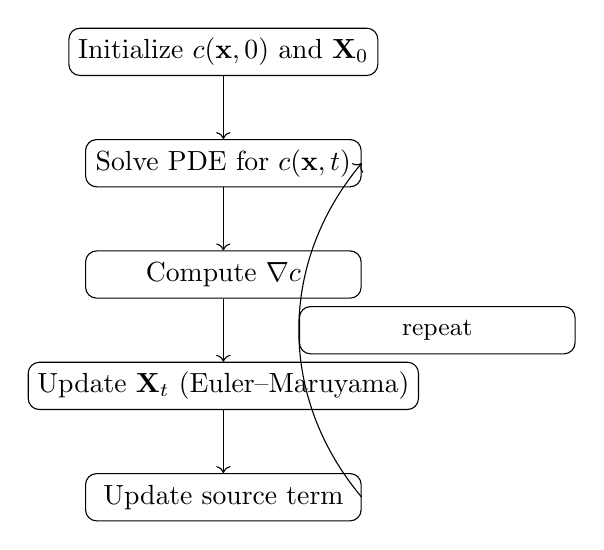
\begin{tikzpicture}[node distance=0.8cm,
				every node/.style={
						draw,
						rounded corners,
						align=center,
						minimum width=3.5cm,
						minimum height=0.6cm}]

			\node (init) {Initialize $c(\mathbf{x},0)$ and $\mathbf{X}_0$};
			\node (pde) [below=of init] {Solve PDE for $c(\mathbf{x},t)$};
			\node (grad) [below=of pde] {Compute $\nabla c$};
			\node (sde) [below=of grad] {Update $\mathbf{X}_t$ (Euler--Maruyama)};
			\node (src) [below=of sde] {Update source term};

			\draw[->] (init)--(pde);
			\draw[->] (pde)--(grad);
			\draw[->] (grad)--(sde);
			\draw[->] (sde)--(src);
			\draw[->,bend left=40] (src.east) to node[right] {\small repeat} (pde.east);

		\end{tikzpicture}

		\column{0.55\textwidth}

		\begin{block}{Key Steps}
			\begin{itemize}
				\item Evolve the chemical field using the diffusion PDE.
				\item Compute the gradient-induced drift.
				\item Update droplet position via Euler--Maruyama and refresh the source term.
			\end{itemize}
		\end{block}

		\begin{alertblock}{Outcome}
			Simultaneous evolution of the chemical field and droplet trajectory generates the simulated paths.
		\end{alertblock}

	\end{columns}

\end{frame}
% %================================================
% \begin{frame}{Simulation Algorithm}

% 	\begin{enumerate}
% 		\item Initialize the droplet position \(\mathbf{X}_0\) and concentration field \(c(\mathbf{x},0)\).
% 		\item Solve the diffusion equation for the concentration field using finite element discretization.
% 		\item Compute the chemical-gradient-induced drift term from the concentration field.
% 		\item Update the droplet position using the Euler--Maruyama scheme.
% 		\item Update the source term according to the new droplet position.
% 		\item Repeat the procedure for all time steps.
% 	\end{enumerate}

% 	\vspace{0.4cm}

% 	\begin{block}{Outcome}
% 		This coupled procedure evolves both the concentration field and the droplet trajectory simultaneously.
% 	\end{block}

% \end{frame}

%================================================
\begin{frame}{Comparison Between Experiment and Simulation}

	\begin{alertblock}{Ensemble Analysis Procedure}

		\begin{itemize}

			\item MSD, VACF, and OCF were computed for each retained trajectory.

			\item Lag times were restricted to approximately
			      $40\%$ of the trajectory length to ensure reliable statistics.

			\item Ensemble observables were obtained by averaging over all retained droplets.

			\item MSD exponents were obtained from
			      $\mathrm{MSD}(\tau)\sim\tau^\alpha$
			      using the first $30\%$ of the available lag-time range.
			\item Exponential fits to VACF and OCF were used
			      to estimate characteristic persistence times
			      $\tau_p$ and $\tau_r$.
			\item Exponential fits
			      $C_v(\tau)\sim e^{-\tau/\tau_p}$ and
			      $C_\theta(\tau)\sim e^{-\tau/\tau_r}$
			      yielded $\tau_p$ and $\tau_r$.

		\end{itemize}

	\end{alertblock}


\end{frame}
%================================================

%================================================
\section{Results and Discussion}

%================================================
\subsection{Ensemble}
%================================================
\begin{frame}{Ensemble Trajectory Comparison}
	\vspace{-0.2cm}
	\begin{columns}[T]

		\column{0.48\textwidth}

		\centering
		\textbf{Experiment}

		\vspace{0.15cm}
		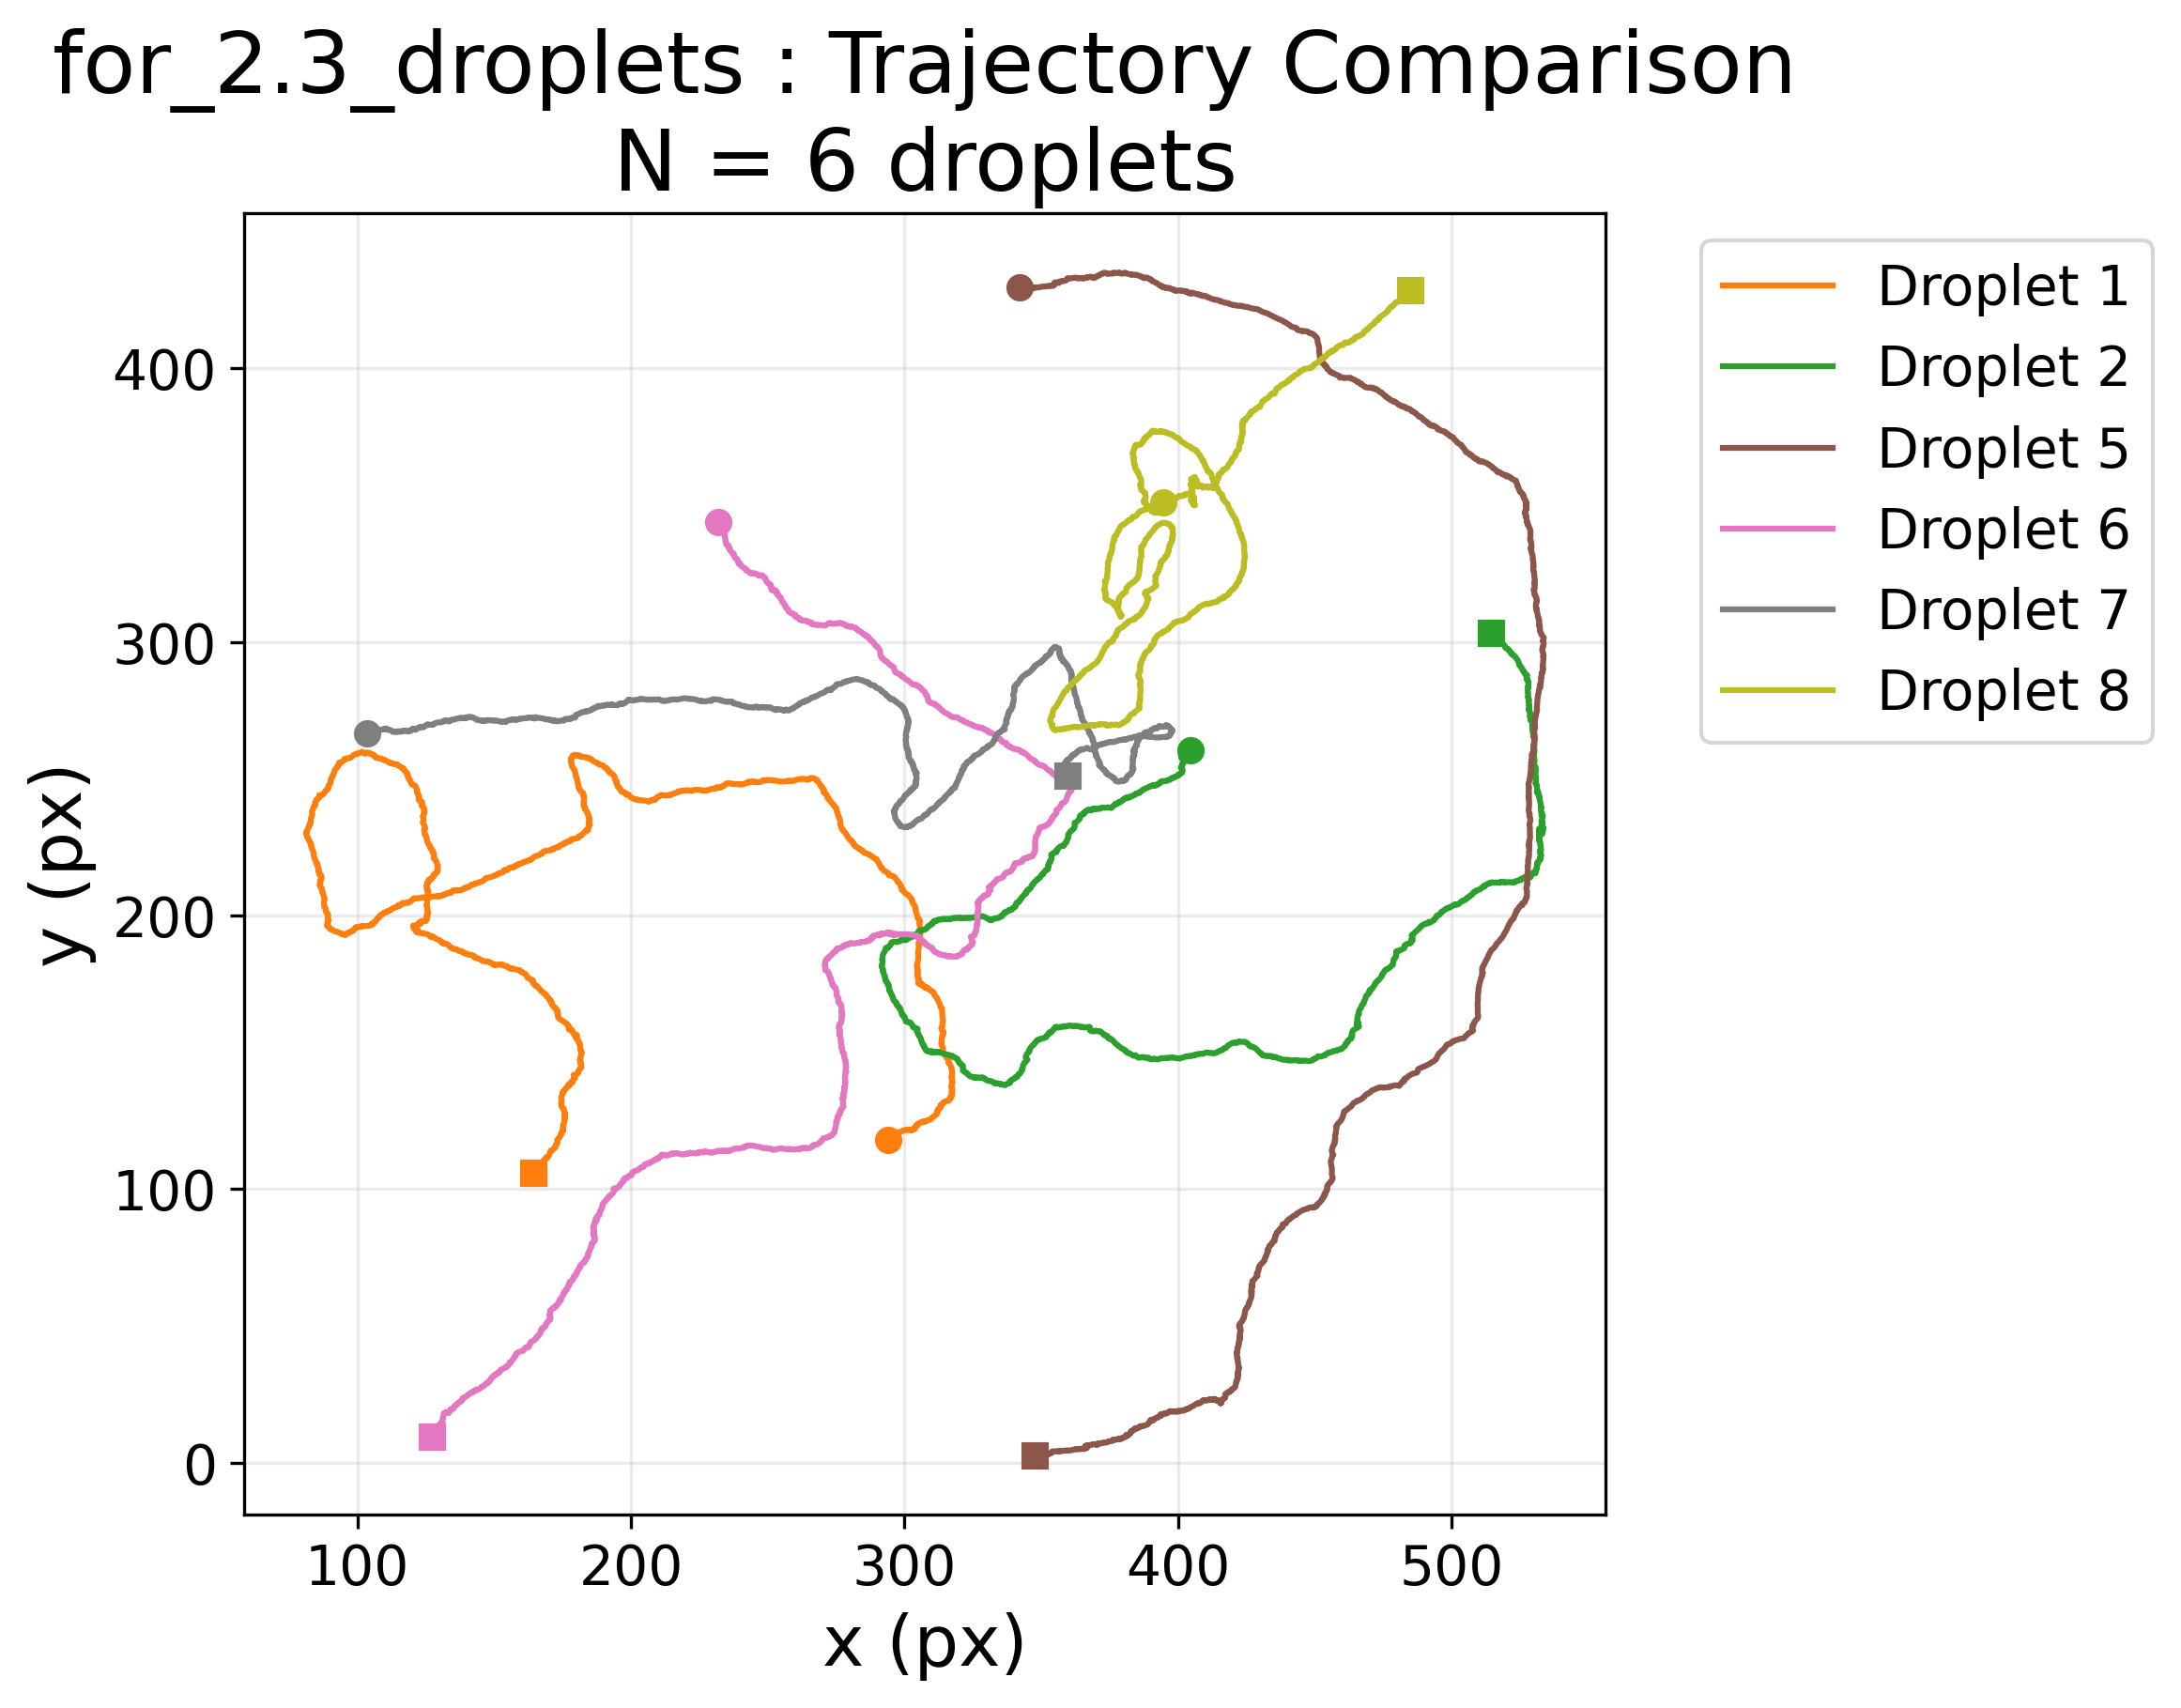
\includegraphics[height=0.62\textheight]{for_2.3_droplets_all_droplets_trajectory_comparison.png}
		\column{0.48\textwidth}

		\centering
		\textbf{Simulation}

		\vspace{0.15cm}

		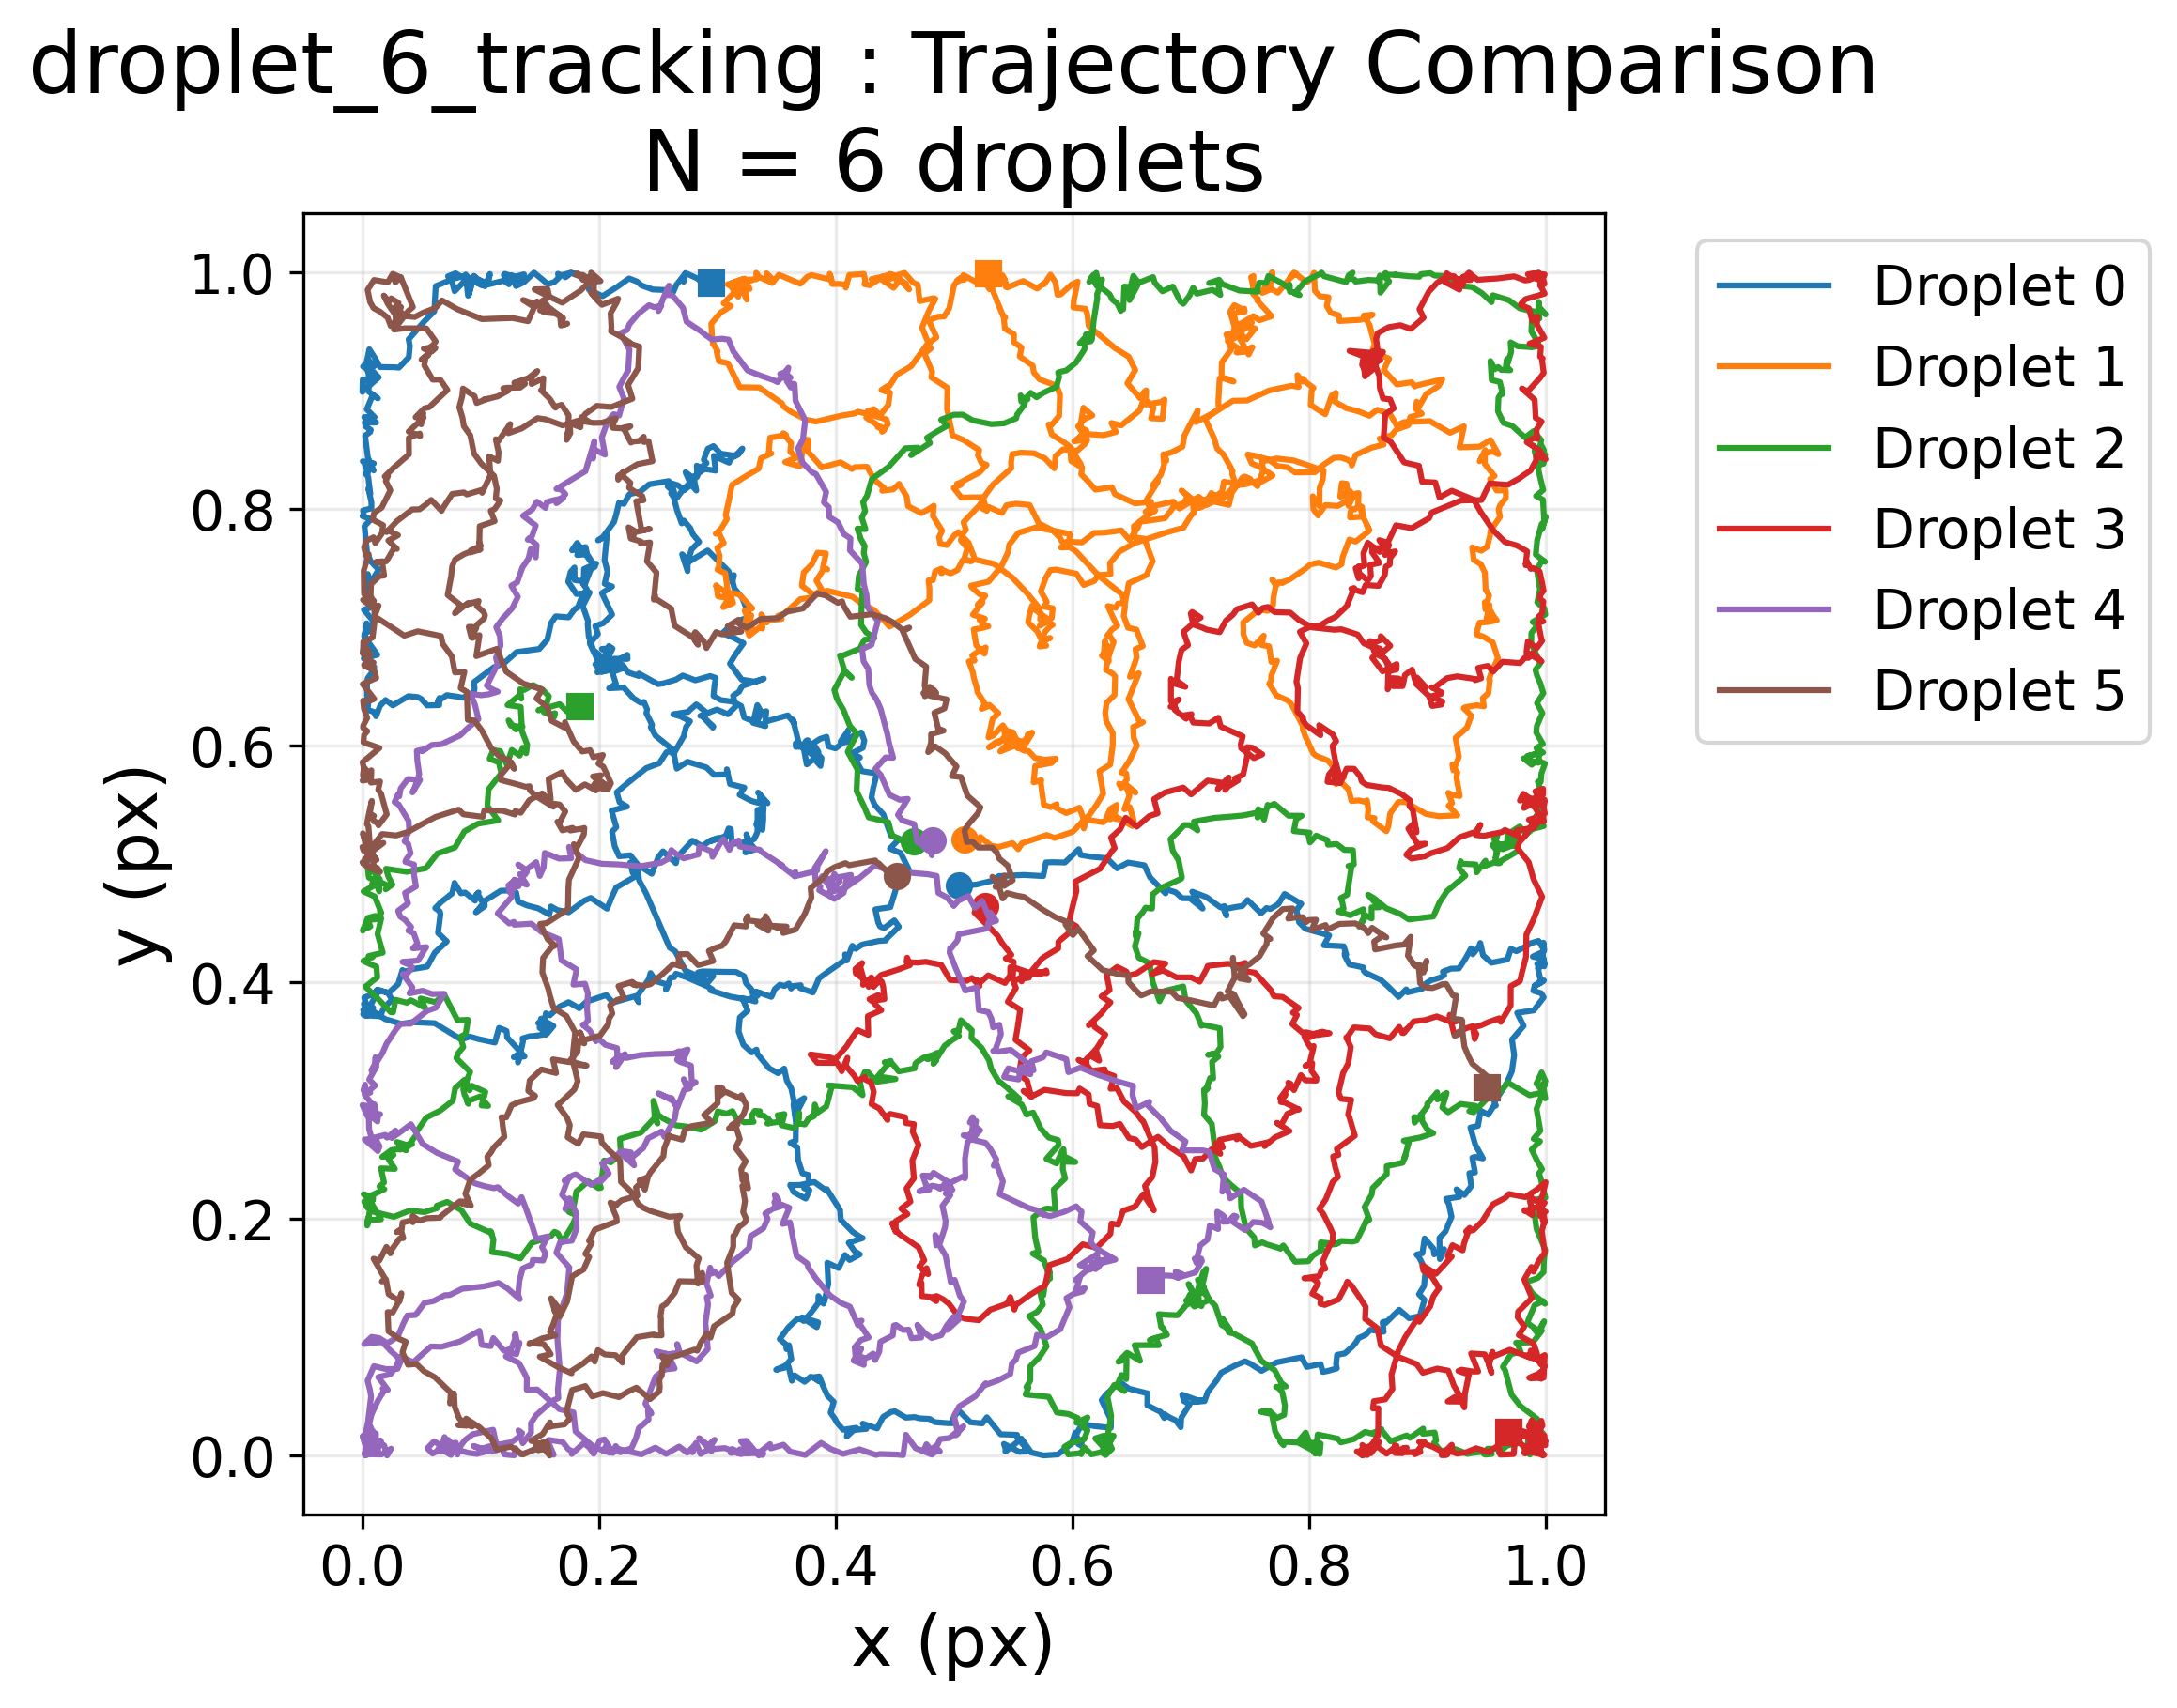
\includegraphics[height=0.62\textheight]{output_sim_droplet_6_tracking_all_droplets_trajectory_comparison.png}

	\end{columns}

	\vspace{0.25cm}

	\centering
	\small

	Persistent exploration and self-avoiding behaviour are observed in both datasets.
	The trajectory start and end positions are indicated by
	$\circ$ and $\blacksquare$, respectively.

\end{frame}

%================================================
\begin{frame}{Ensemble Mean-Squared Displacement}

	\begin{columns}[T]

		%------------------------------------------------
		\column{0.48\textwidth}

		\centering
		\textbf{Experiment}

		% \vspace{-0.05cm}

		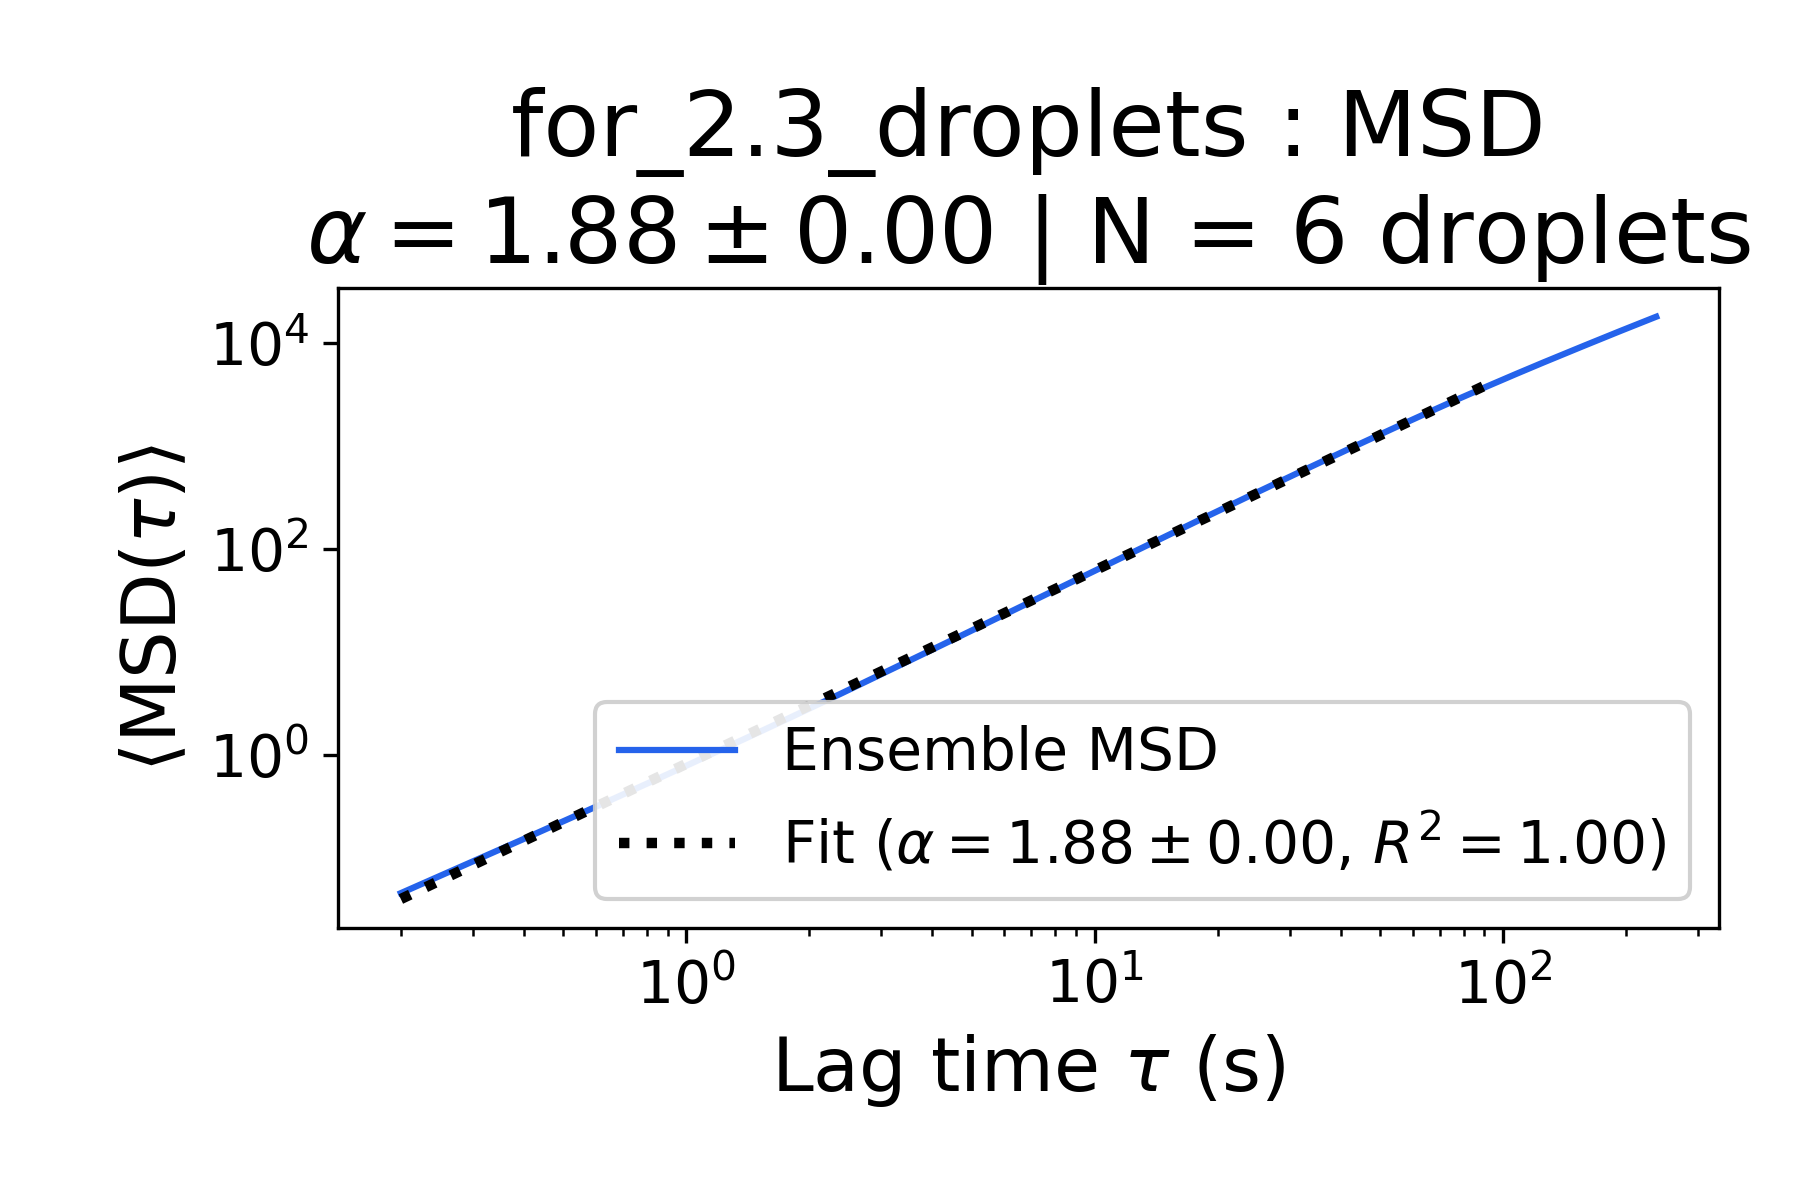
\includegraphics[height=0.52\textheight]{for_2.3_droplets_ensemble_for_2.3_droplets_loglog_msd.png}

		\vspace{-0.1cm}

		{\small
			$\alpha = 1.88 \pm 0.00$
		}

		%------------------------------------------------
		\column{0.48\textwidth}

		\centering
		\textbf{Simulation}

		% \vspace{0.15cm}
		% \vspace{-0.15cm}

		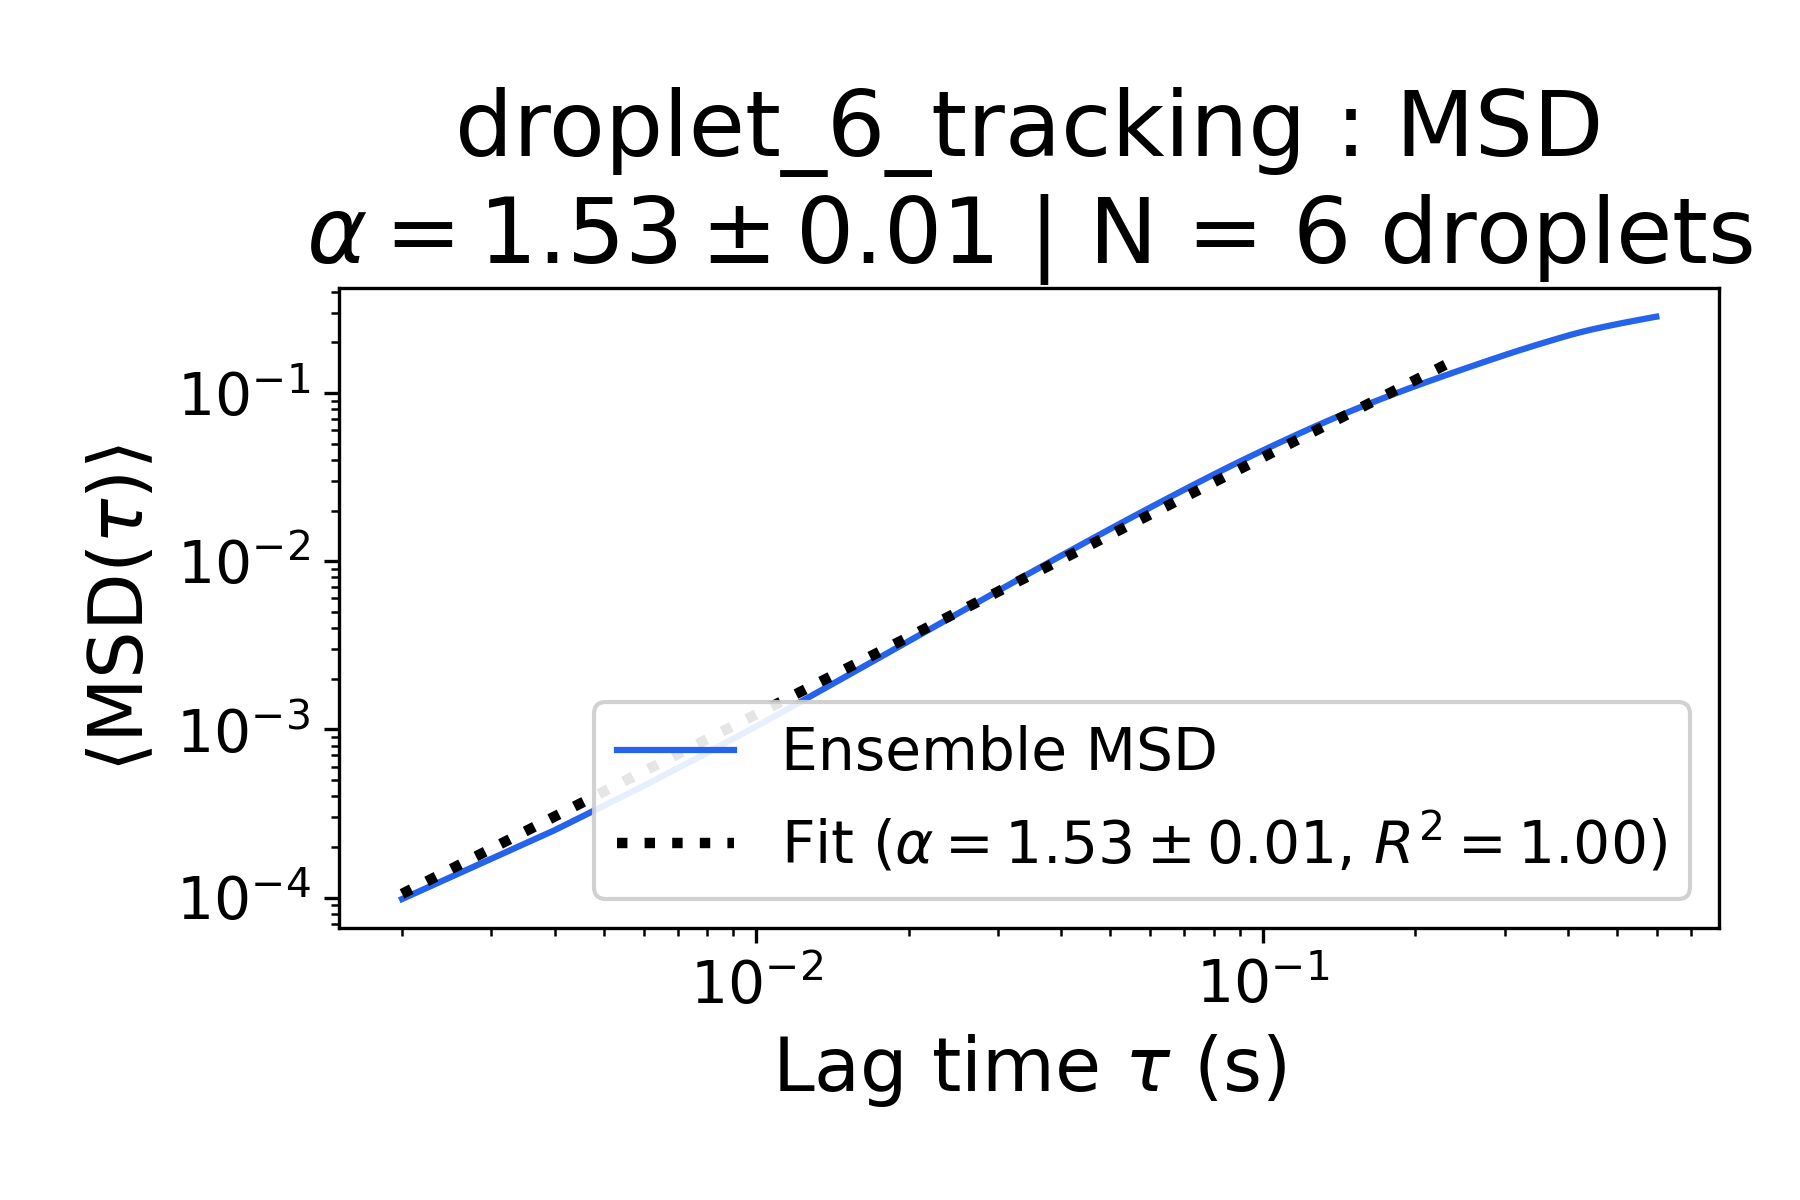
\includegraphics[height=0.52\textheight]{output_sim_ensemble_droplet_6_tracking_loglog_msd.png}

		\vspace{-0.1cm}

		{\small
			$\alpha = 1.53 \pm 0.01$
		}

	\end{columns}

	\vspace{-0.1cm}

	\begin{alertblock}{Key Observation}
		Both datasets exhibit superdiffusive transport ($\alpha > 1$), indicating persistent motion and departure from normal diffusion.
	\end{alertblock}

\end{frame}


%================================================
\begin{frame}{Ensemble Velocity Autocorrelation Function}
	\vspace{-0.2cm}

	\begin{columns}[T]

		%------------------------------------------------
		\column{0.48\textwidth}

		\centering
		\textbf{Experiment}

		\vspace{0.15cm}

		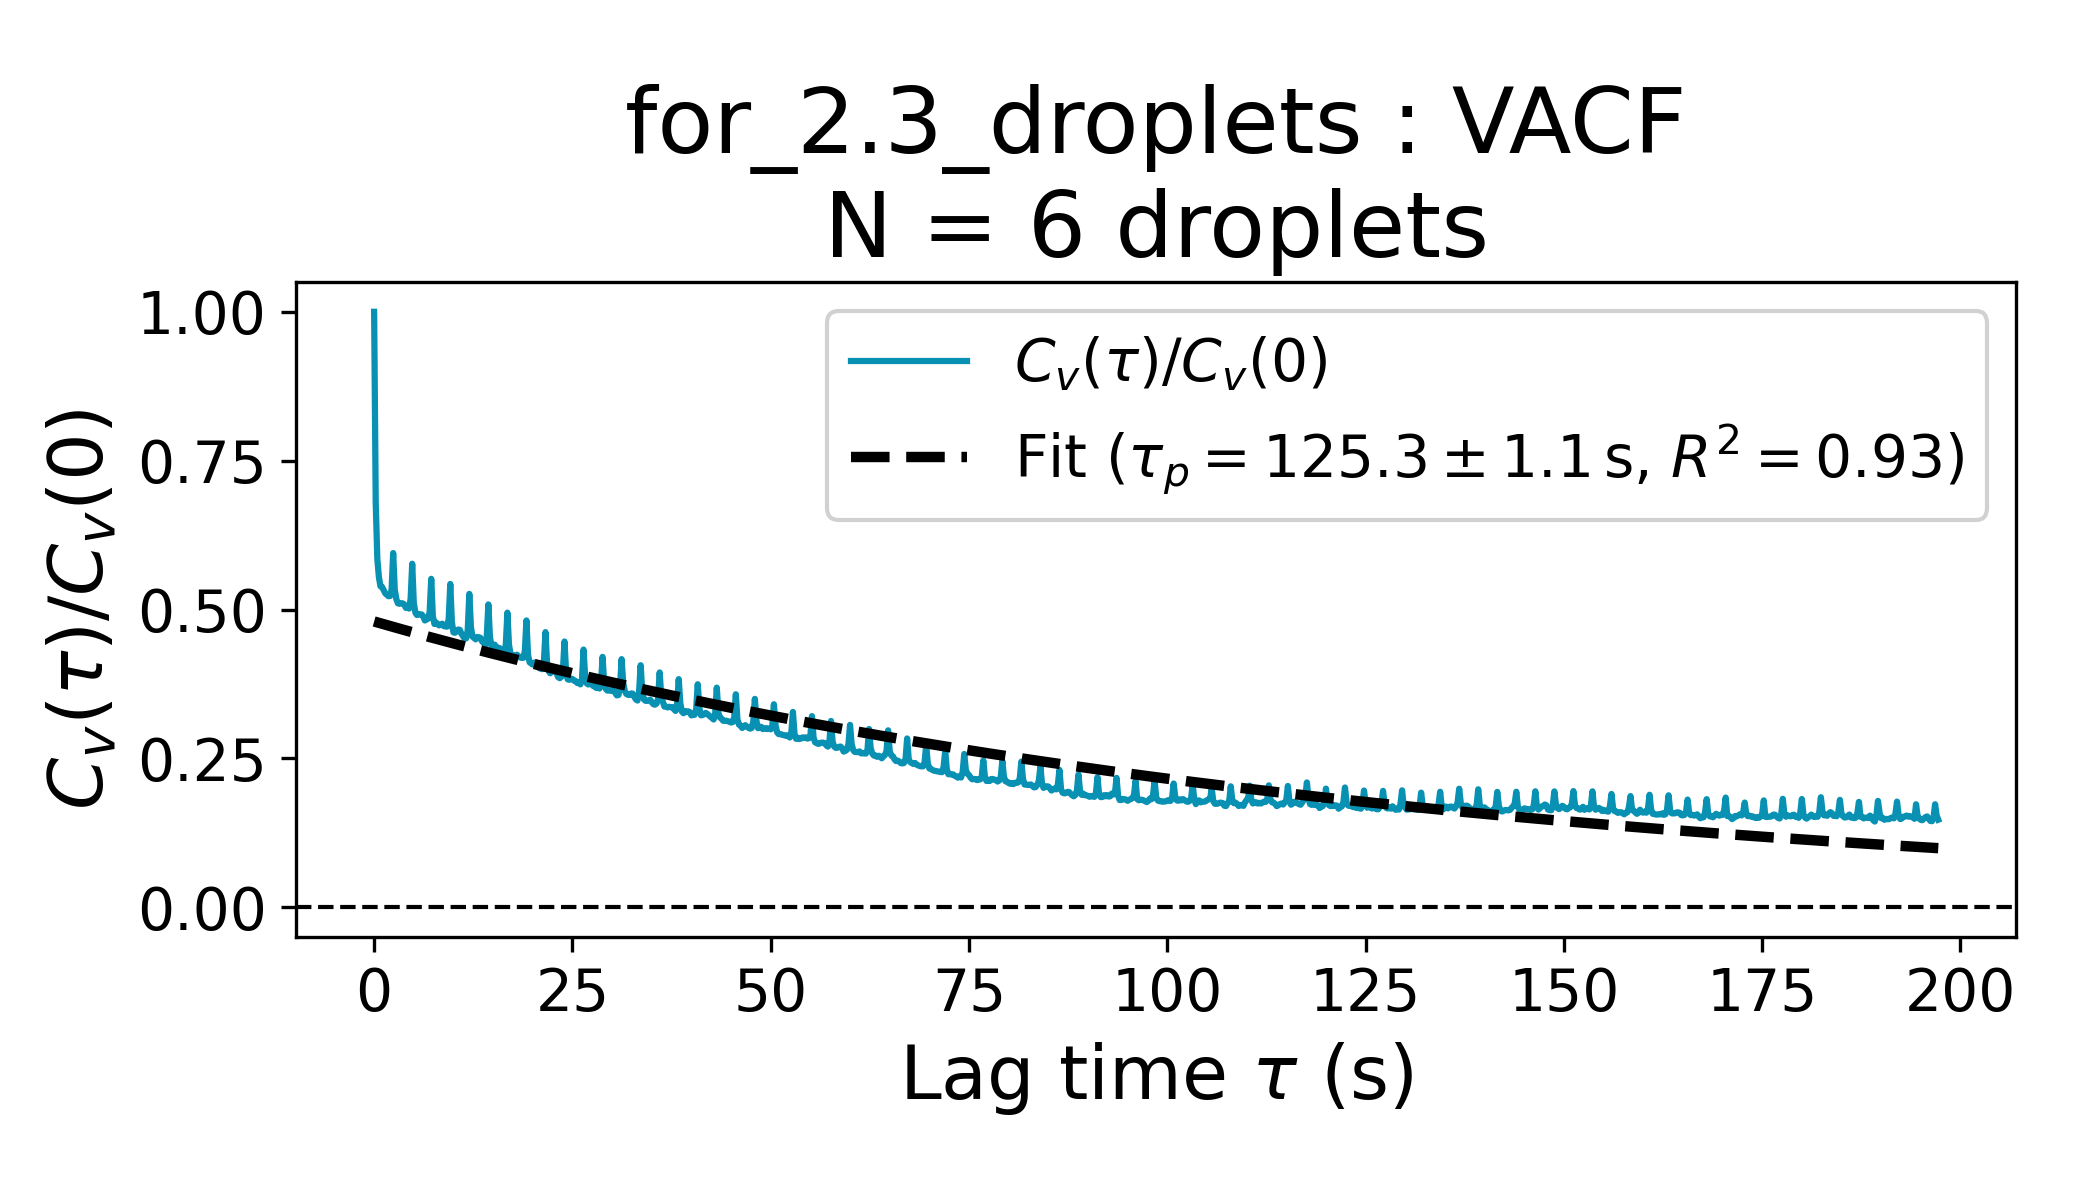
\includegraphics[width=\linewidth]{for_2.3_droplets_ensemble_for_2.3_droplets_vacf.png}

		\vspace{0.1cm}

		{\small
			$\tau_p = 125.3 \pm 11.1~\mathrm{s}$
		}

		%------------------------------------------------
		\column{0.48\textwidth}

		\centering
		\textbf{Simulation}

		\vspace{0.15cm}

		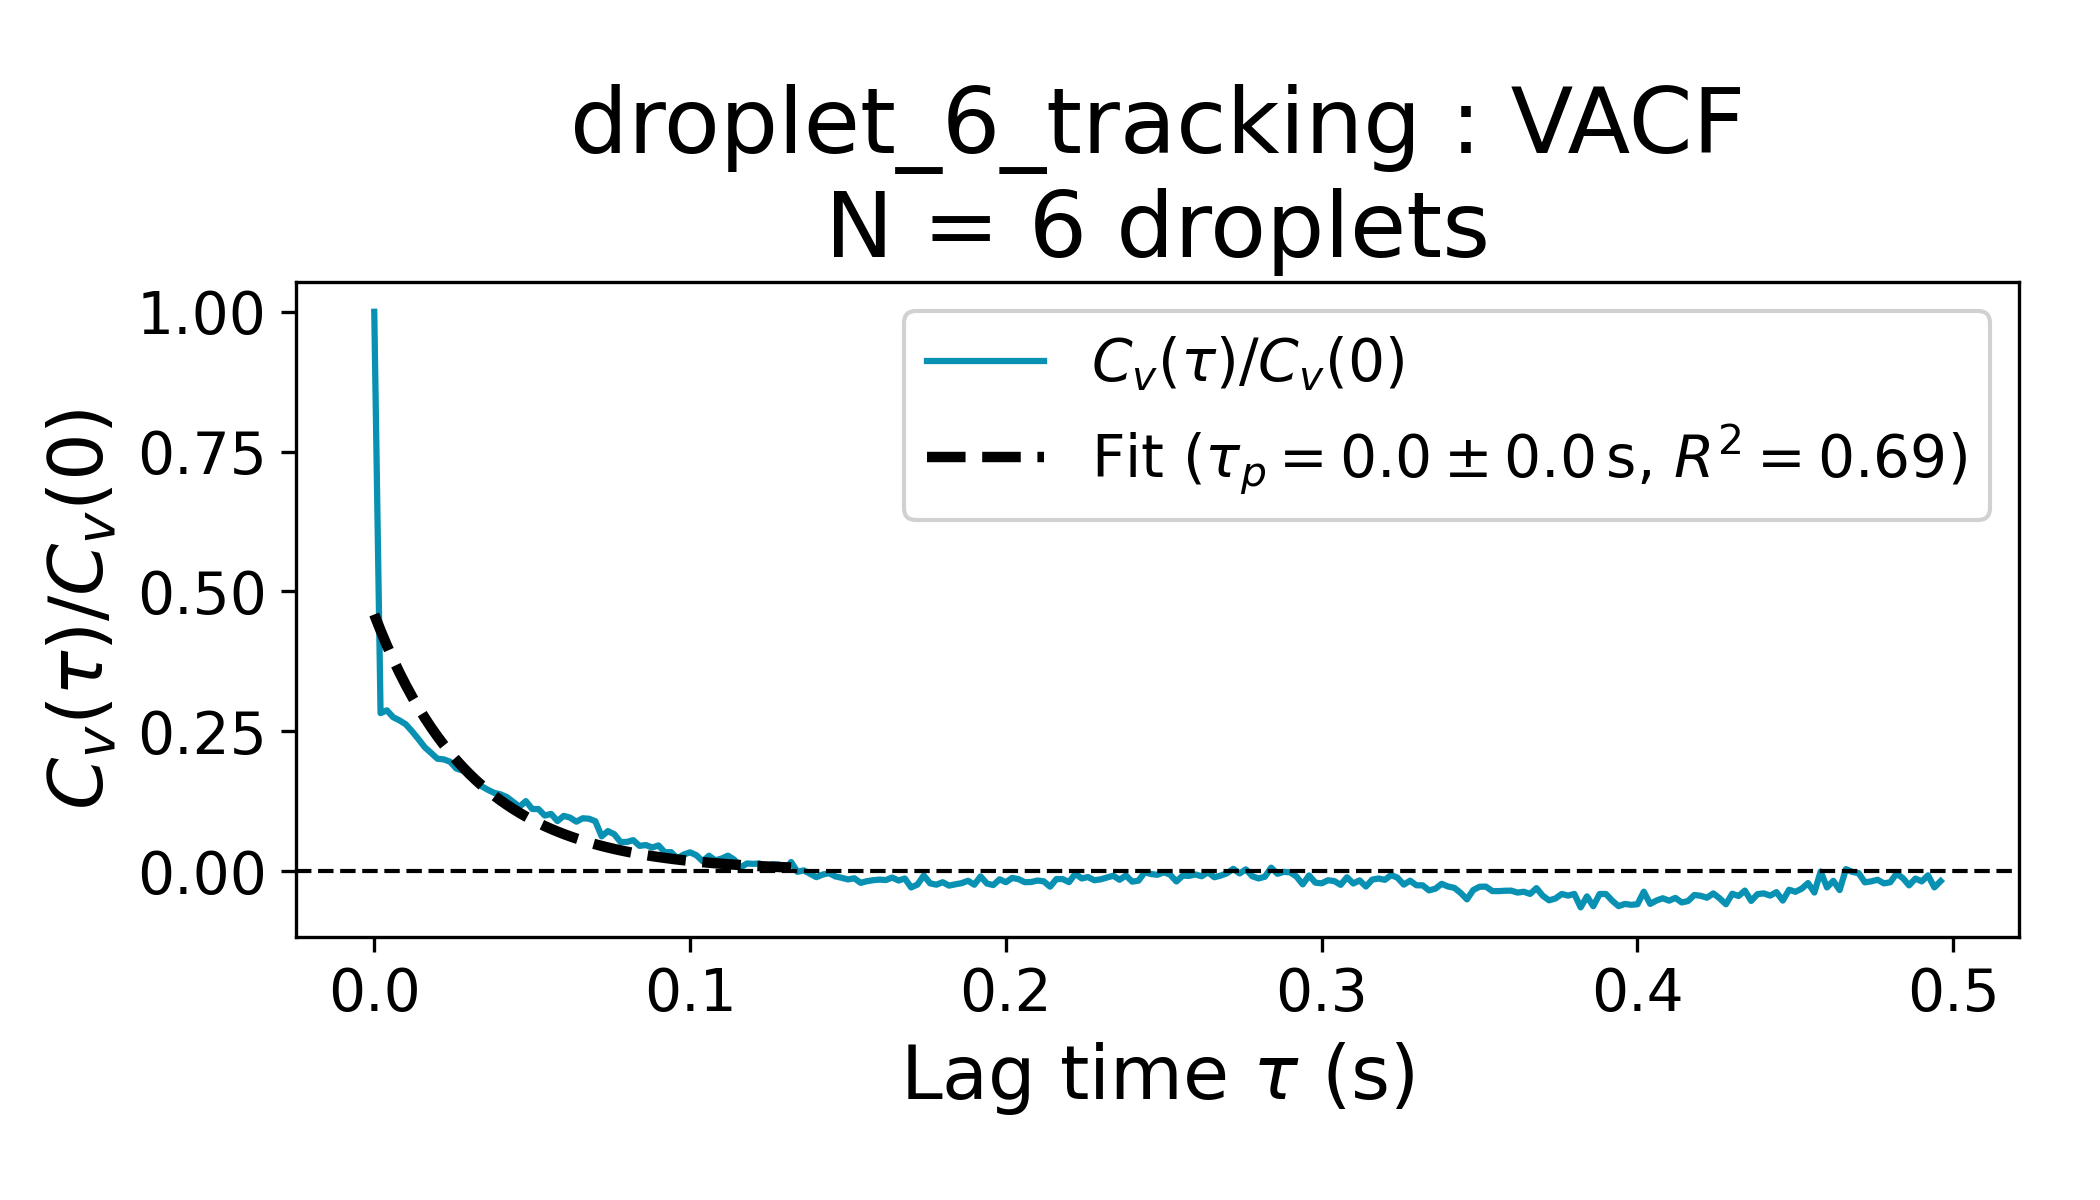
\includegraphics[width=\linewidth]{output_sim_ensemble_droplet_6_tracking_vacf.png}

		\vspace{0.1cm}

		{\small
			$\tau_p = 0.031 \pm 0.004$
		}

	\end{columns}

	\vspace{0.2cm}

	\begin{alertblock}{Key Observation}
		Both VACFs decay over a finite timescale, indicating persistent velocity correlations and finite translational memory.
	\end{alertblock}

\end{frame}
%================================================
\begin{frame}{Ensemble Orientation Correlation Function}

	\begin{columns}[T]

		%------------------------------------------------
		\column{0.48\textwidth}

		\centering
		\textbf{Experiment}

		\vspace{0.15cm}

		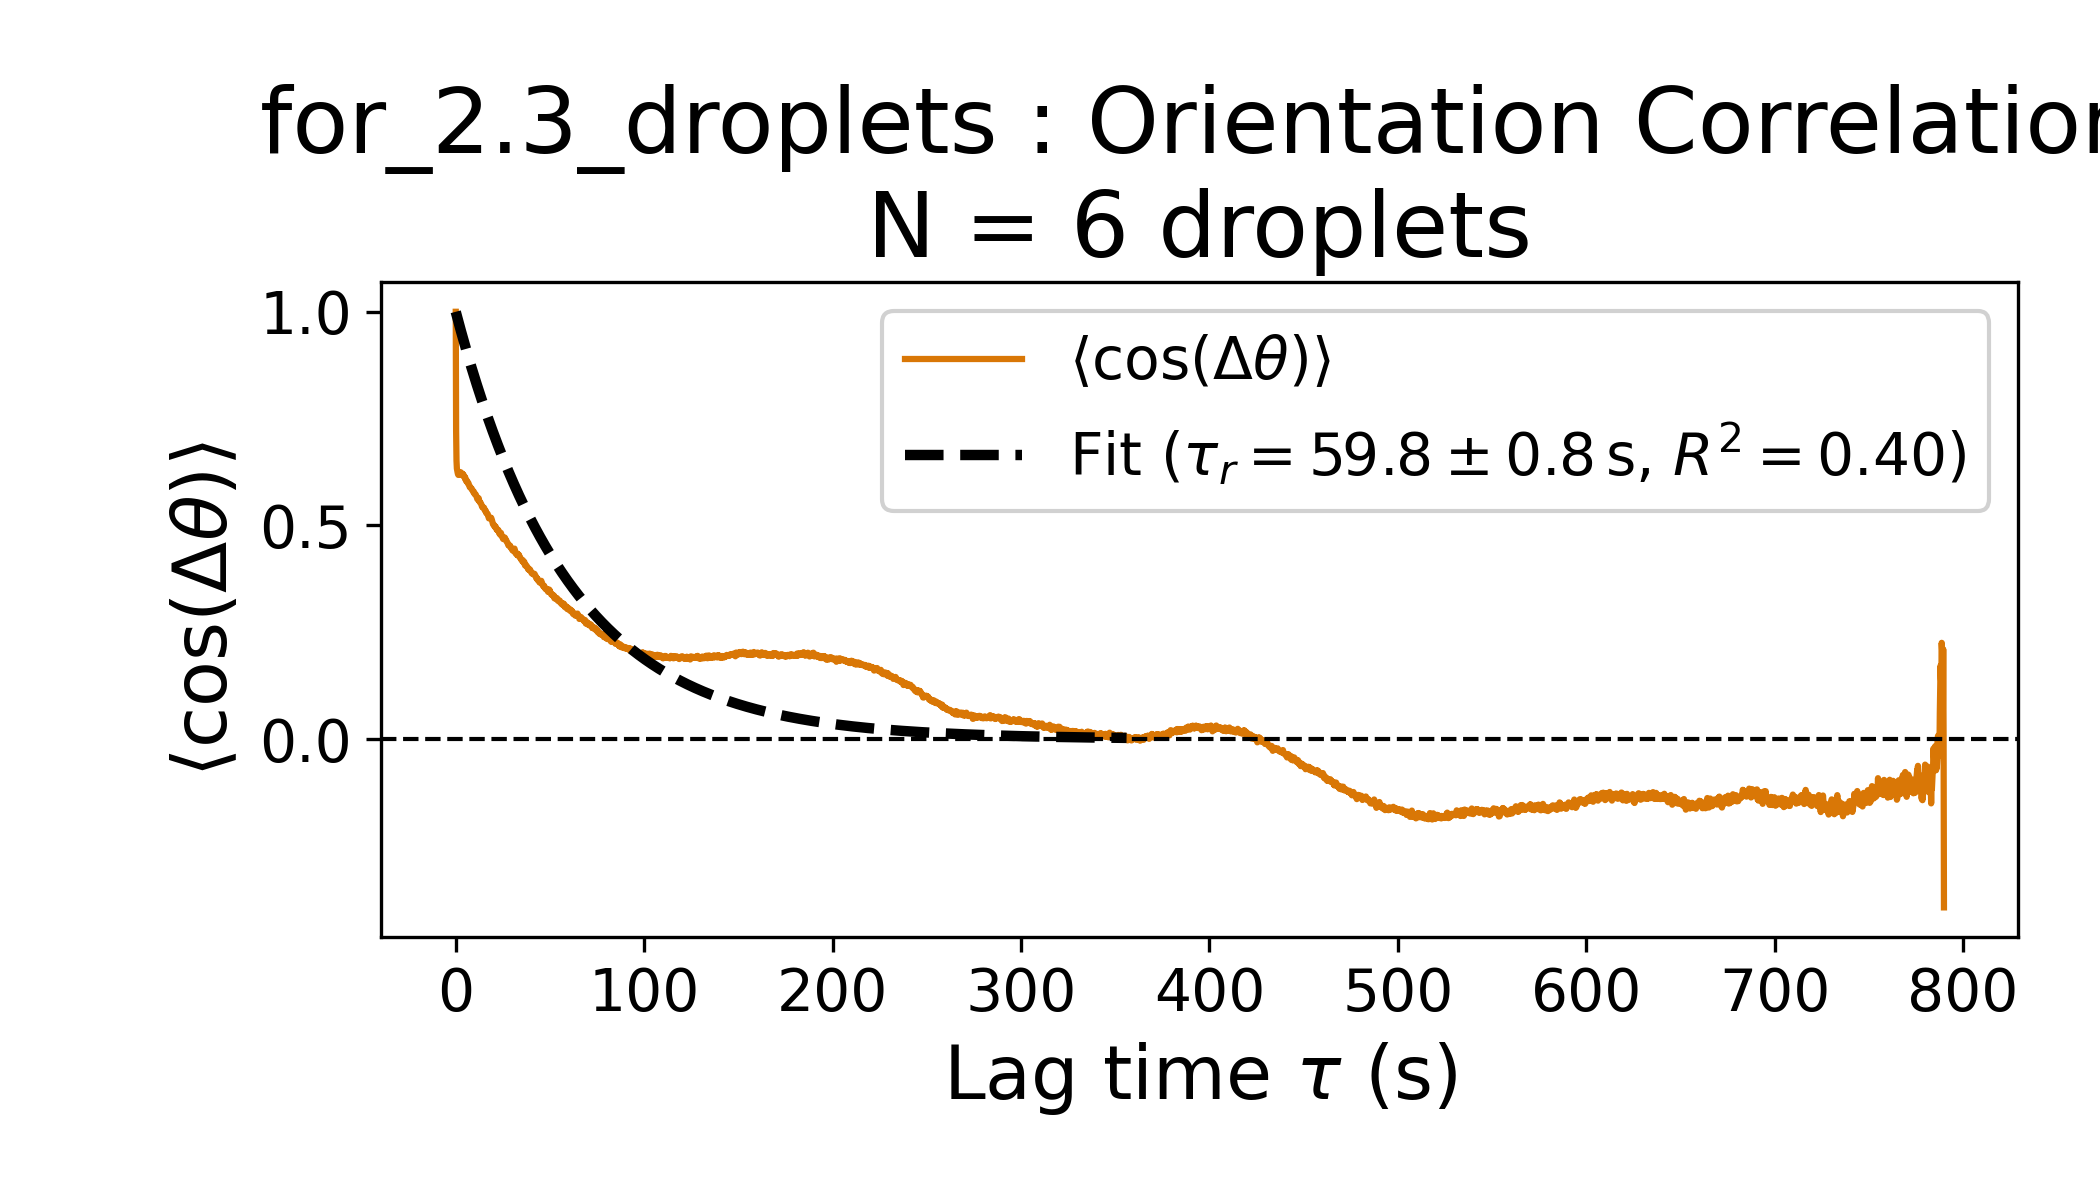
\includegraphics[width=\linewidth]{for_2.3_droplets_ensemble_for_2.3_droplets_orientation_corr.png}

		\vspace{0.1cm}

		{\small
			$\tau_r = 59.8 \pm 0.8~\mathrm{s}$
		}

		%------------------------------------------------
		\column{0.48\textwidth}

		\centering
		\textbf{Simulation}

		\vspace{0.15cm}

		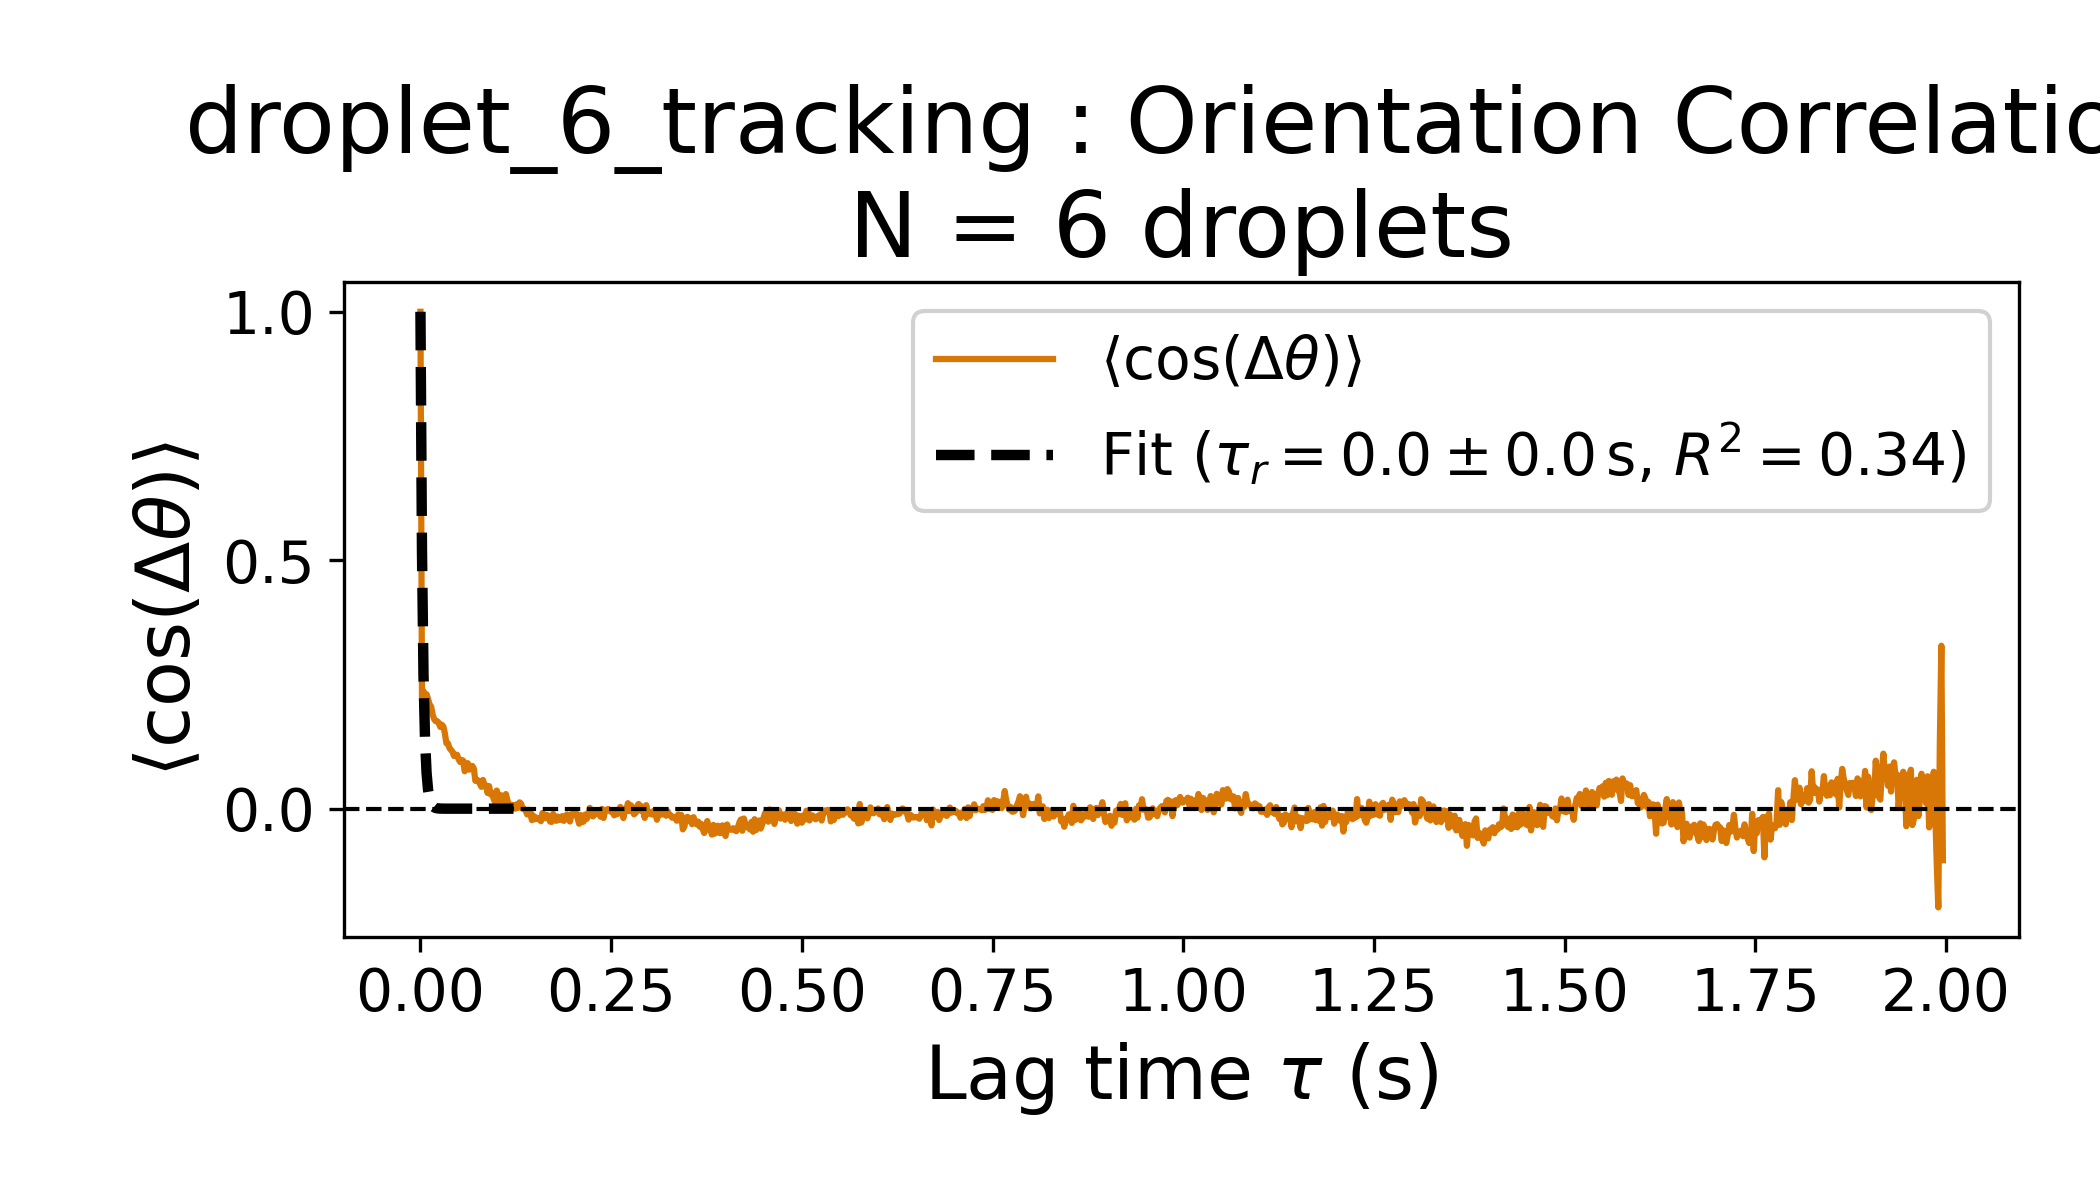
\includegraphics[width=\linewidth]{output_sim_ensemble_droplet_6_tracking_orientation_corr.png}

		\vspace{0.1cm}

		{\small
			$\tau_r = 0.00305 \pm 0.00054$
		}

		% If using scaled values instead:
		% {\small
		% $\tau_r = 0.00305 \pm 0.00054$
		%
		% $\tau_r^{(\mathrm{scaled})}
		% =
		% 1.41 \pm 0.25~\mathrm{s}$
		% }

	\end{columns}

	\vspace{0.2cm}

	\begin{alertblock}{Key Observation}
		The orientation correlations decay gradually in both experiment and simulation, indicating finite directional persistence and rotational memory.
	\end{alertblock}

\end{frame}
%================================================

%================================================
\begin{frame}{Summary of Ensemble Transport Parameters}

	\centering
	\scriptsize

	\begin{table}
		\centering
		\begin{tabular}{lcccccc}
			\toprule
			Dataset      &
			$N$          &
			Frames /
			Iterations   &
			$\alpha$     &
			$\tau_p$ (s) &
			$\tau_r$ (s)                         \\
			\midrule

			2.1
			             & 4
			             & 3648
			             & $1.8345 \pm 0.0019$
			             & $61.83 \pm 0.36$
			             & $13.49 \pm 0.34$
			\\

			2.2
			             & 6
			             & 3363
			             & $1.6482 \pm 0.0053$
			             & $17.14 \pm 0.56$
			             & $3.96 \pm 0.26$
			\\

			2.3
			             & 6
			             & 3951
			             & $1.8776 \pm 0.0012$
			             & $125.25 \pm 1.09$
			             & $59.78 \pm 0.78$
			\\

			2.4
			             & 3
			             & 5267
			             & $1.7025 \pm 0.0049$
			             & $28.40 \pm 0.22$
			             & $32.18 \pm 0.35$
			\\

			2\&4 $\mu$L
			             & 4
			             & 5526
			             & $1.5592 \pm 0.0066$
			             & $14.32 \pm 0.16$
			             & $10.83 \pm 0.20$
			\\

			\midrule

			Simulation
			             & 6
			             & 1000
			             & $1.5272 \pm 0.0088$
			             & $0.0310 \pm 0.0036$
			             & $0.00305 \pm 0.00054$
			\\

			Simulation (Scaled)
			             & 6
			             & 1000
			             & $1.5272 \pm 0.0088$
			             & $14.32 \pm 1.66$
			             & $1.41 \pm 0.25$
			\\

			\bottomrule
		\end{tabular}
	\end{table}

	\vspace{0.2cm}

	{\tiny
		Simulation persistence times were converted using
		$t_{\mathrm{scale}}
			=
			\tau_p^{\mathrm{exp}}
			/
			\tau_p^{\mathrm{sim}}
			\approx 462$.
	}

	\begin{alertblock}{Key Observation}
		The model reproduces the superdiffusive transport exponent
		($\alpha>1$) and exhibits finite velocity and directional persistence,
		consistent with memory-driven dynamics.
	\end{alertblock}

\end{frame}

\begin{frame}{Experiment--Simulation Comparison}

	\centering

	\begin{tabular}{lcc}
		\toprule
		Feature                     & Experiment   & Simulation   \\
		\midrule
		Self-avoidance              & $\checkmark$ & $\checkmark$ \\
		Superdiffusion ($\alpha>1$) & $\checkmark$ & $\checkmark$ \\
		VACF decay                  & $\checkmark$ & Partial      \\
		OCF decay                   & $\checkmark$ & Partial      \\
		Translational memory        & $\checkmark$ & Partial      \\
		Rotational memory           & $\checkmark$ & Partial      \\
		Non-Markovian behaviour     & $\checkmark$ & Qualitative  \\
		\bottomrule
	\end{tabular}

	\vspace{0.2cm}
	\begin{minipage}{0.9\linewidth}
		\footnotesize
		\textbf{Limitation:}
		The simulation reproduces the qualitative decay of the VACF and OCF,
		but the persistence times ($\tau_p,\tau_r$) differ substantially from
		the experimental values.
	\end{minipage}
	% \textbf{Conclusion:}
	\begin{alertblock}{Conclusion}
		The PDE--SDE model captures the key transport and memory signatures
		(self-avoidance, superdiffusion, and finite correlation decay),
		but does not quantitatively reproduce the experimental persistence times.
		% 	The PDE--SDE model reproduces the main transport and memory signatures observed experimentally.
	\end{alertblock}

\end{frame}

%================================================
% \subsection{Summary of Results}

% \begin{frame}{Summary of Results}

% 	\begin{itemize}
% 		\item The experimental trajectories show self-avoiding motion.
% 		\item The MSD indicates superdiffusive transport.
% 		\item The local MSD exponent reveals a change in transport regime with lag time.
% 		\item The VACF and OCF show finite velocity and directional persistence.
% 		\item The coupled PDE--SDE model reproduces the main qualitative trends seen in experiment.
% 	\end{itemize}

% 	\vspace{0.3cm}

% 	\begin{alertblock}{Main Conclusion}
% 		The simulation captures the observed self-avoidance, transport scaling, and finite memory timescales.
% 	\end{alertblock}

% \end{frame}

\section{Conclusion}
%================================================
\begin{frame}{Conclusions}

	\begin{block}{Main Findings}
		\begin{itemize}
			\item Experimental droplet trajectories exhibit persistent self-avoiding motion.

			\item MSD analysis indicates superdiffusive transport
			      ($\alpha > 1$).

			\item VACF and OCF reveal finite translational
			      ($\tau_p$) and rotational ($\tau_r$) memory.

			\item A memory-driven PDE--SDE model was developed
			      based on droplet--chemical field interactions.

			\item The model reproduces the key qualitative
			      transport and memory signatures observed experimentally.
		\end{itemize}
	\end{block}

	\begin{alertblock}{Key Limitation}
		The model reproduces the qualitative decay of the VACF and OCF,
		but significantly underestimates the persistence times
		($\tau_p,\tau_r$) measured experimentally.
	\end{alertblock}

\end{frame}
%================================================
% \begin{frame}{Future Work}

% 	\begin{itemize}

% 		\item Calibrate model parameters using experimental measurements
% 		      to enable quantitative comparison.

% 		      \vspace{0.2cm}

% 		\item Investigate alternative memory kernels and generalized
% 		      Langevin descriptions.

% 		      \vspace{0.2cm}

% 		\item Study collective behaviour and interactions between multiple
% 		      active droplets.

% 		      \vspace{0.2cm}

% 		\item Extend the framework to other memory-driven active matter
% 		      systems.

% 		      \vspace{0.2cm}

% 		\item Explore long-time transport and anomalous diffusion regimes.

% 	\end{itemize}

% 	\vspace{0.5cm}

% 	\begin{alertblock}{Long-Term Goal}
% 		Develop predictive memory-driven models for active matter systems
% 		that couple stochastic motion with evolving environmental fields.
% 	\end{alertblock}

% \end{frame}

\begin{frame}{Outlook and Future Work}

	\begin{block}{Physical Interpretation}
		The results support the hypothesis that active droplet
		motion is influenced by memory effects arising from
		self-generated chemical fields, leading to
		history-dependent dynamics.
	\end{block}

	\begin{block}{Future Directions}
		\begin{itemize}
			\item Calibrate model parameters for quantitative agreement.

			\item Investigate memory-kernel based descriptions
			      (e.g., Generalized Langevin Equation).

			\item Extend the framework to interacting droplets
			      and collective behaviour.

			\item Explore long-time transport and anomalous
			      diffusion regimes.
		\end{itemize}
	\end{block}

	\begin{alertblock}{Long-Term Goal}
		Develop predictive memory-driven models for active matter
		systems that couple stochastic motion with evolving
		environmental fields.
	\end{alertblock}

\end{frame}


\begin{frame}[allowframebreaks]{References}
	\printbibliography
\end{frame}

\end{document}
